\setcounter{chapter}{0}
\chapter{Dal determinismo al calcolo quantistico}
\phantomsection\label{chapter-1}

Dai dati iniziali di un sistema alle ampiezze: seguiamo le informazioni necessarie per costruire una simulazione.\par


\clearpage\phantomsection\label{exercise-index-1}
\BookHeading{Percorso degli esercizi guidati}
Quindici esercizi accompagnano lo studio del modulo. Ogni traccia segue le sezioni richieste e rinvia a uno svolgimento completo. Si suggerisce di formulare la previsione e tentare i passaggi prima di consultare la soluzione.
\begin{longtable}{@{}p{13mm}p{75mm}r@{}}\toprule Codice & Argomento & Pagina\\\midrule\endhead
\hyperref[ex-G1.01]{G1.01} & Prevedere due moti dagli stessi dati di posizione & \pageref{ex-G1.01}\\[3pt]
\hyperref[ex-G1.02]{G1.02} & Propagare un'incertezza sulla velocità & \pageref{ex-G1.02}\\[3pt]
\hyperref[ex-G1.03]{G1.03} & Invertire un moto e ritrovare la preparazione & \pageref{ex-G1.03}\\[3pt]
\hyperref[ex-G1.04]{G1.04} & Confrontare ritorno ideale e ritorno perturbato & \pageref{ex-G1.04}\\[3pt]
\hyperref[ex-G1.05]{G1.05} & Sommare due onde con fase assegnata & \pageref{ex-G1.05}\\[3pt]
\hyperref[ex-G1.06]{G1.06} & Dalle ampiezze all'intensità & \pageref{ex-G1.06}\\[3pt]
\hyperref[ex-G1.07]{G1.07} & Localizzare i minimi per una fenditura stretta & \pageref{ex-G1.07}\\[3pt]
\hyperref[ex-G1.08]{G1.08} & Attraversare i regimi della diffrazione & \pageref{ex-G1.08}\\[3pt]
\hyperref[ex-G1.09]{G1.09} & Prevedere la trasmissione di un analizzatore & \pageref{ex-G1.09}\\[3pt]
\hyperref[ex-G1.10]{G1.10} & Seguire una preparazione sulla sfera di Bloch & \pageref{ex-G1.10}\\[3pt]
\hyperref[ex-G1.11]{G1.11} & Preparare, introdurre una fase e ricombinare & \pageref{ex-G1.11}\\[3pt]
\hyperref[ex-G1.12]{G1.12} & Ricavare marginali e correlazioni da una tabella congiunta & \pageref{ex-G1.12}\\[3pt]
\hyperref[ex-G1.13]{G1.13} & Seguire l'effetto di un'interazione con l'ambiente & \pageref{ex-G1.13}\\[3pt]
\hyperref[ex-G1.14]{G1.14} & Stabilire quali dati servano alla previsione successiva & \pageref{ex-G1.14}\\[3pt]
\hyperref[ex-G1.15]{G1.15} & Ricostruire un esperimento a partire dai suoi risultati & \pageref{ex-G1.15}\\[3pt]
\bottomrule\end{longtable}
{\small I primi cinque esercizi offrono una guida esplicita; i successivi cinque consolidano il calcolo; gli ultimi cinque collegano più concetti. Tutti conservano uno svolgimento completo.}\par

\Needspace{.43\textheight}
\section{Dati iniziali e previsione del moto}
\phantomsection\label{c1-moto}

{\sffamily\small\color{Ink!70} Riferimento alle slide: p. 12.\par}

{\sffamily\small\color{Ink!70} Laboratorio locale: \nolinkurl{index.html#capitolo-1/moto}\par}

Due particelle partono dallo stesso punto. Per prevedere dove si troveranno occorre conoscere anche la loro velocità. Il primo confronto segue due moti ben determinati; la raccolta sottostante mostra invece che cosa accade quando i dati della preparazione sono noti soltanto entro un intervallo.\par


\BookHeading{Preparazione e significato dei comandi}

Posizione iniziale\par

È il punto da cui partono sia \(A\) sia \(B\). Il valore 0 è l'origine scelta per misurare le distanze, non un bordo del tavolo.\par

Velocità \(A\)\par

Indica lo spostamento di \(A\) in un secondo. Un valore positivo porta verso destra; un valore negativo verso sinistra; con 0 la particella resta ferma.\par

Velocità \(B\)\par

\(B\) parte dallo stesso punto di \(A\), ma può avere una velocità diversa. I due moti vengono calcolati separatamente.\par

Incertezza sulla velocità \(A\)\par

Specifica quanto la velocità può differire dal valore centrale, in entrambi i versi. Per 3 m/s con incertezza 0,5 m/s consideriamo tutte le velocità da 2,5 a 3,5 m/s.\par


\BookHeading{Figure della configurazione iniziale}
\begin{FigureBlock}\centering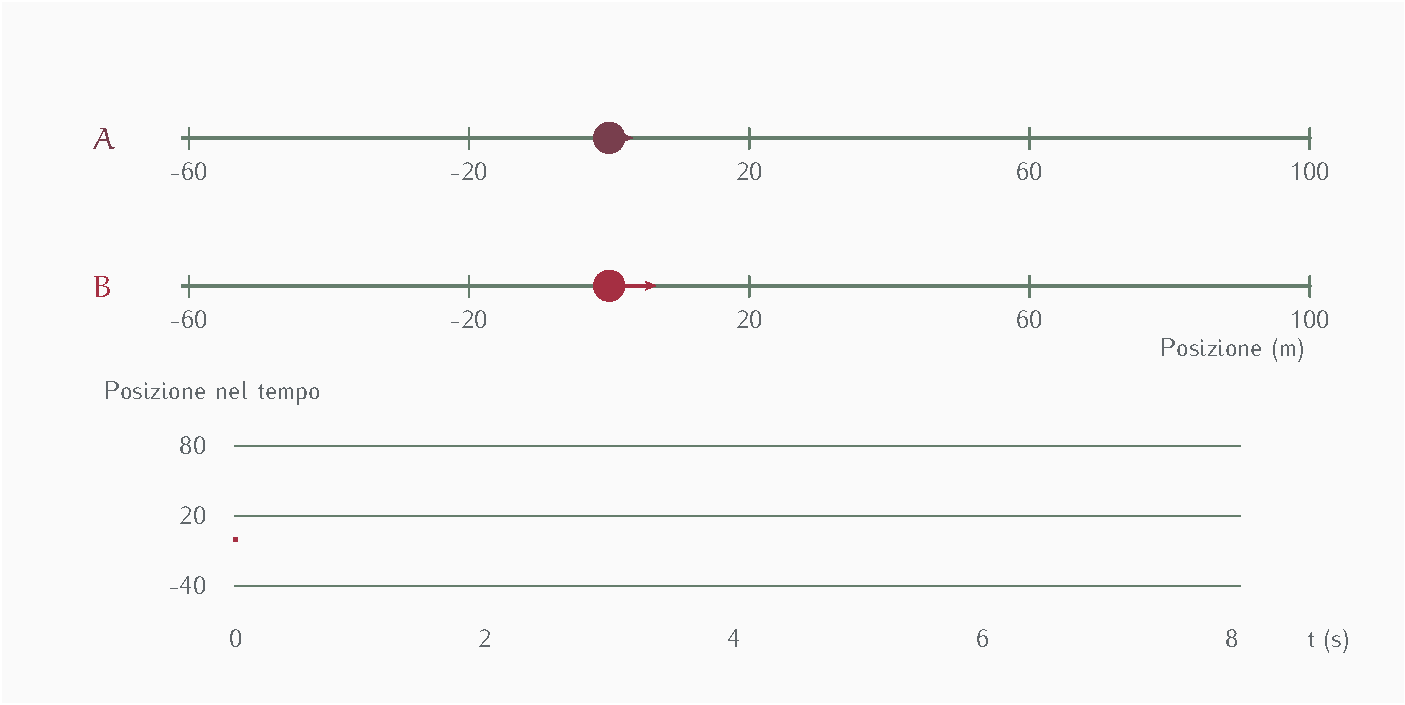
\includegraphics[width=\linewidth,height=94mm,keepaspectratio]{figure/fec498382cb770de3.pdf}\FigureCaption{Due moti uniformi. Tempo 0,0 secondi. \(A\) a 0,0 metri, \(B\) a 0,0 metri.}\end{FigureBlock}
\begin{FigureBlock}\centering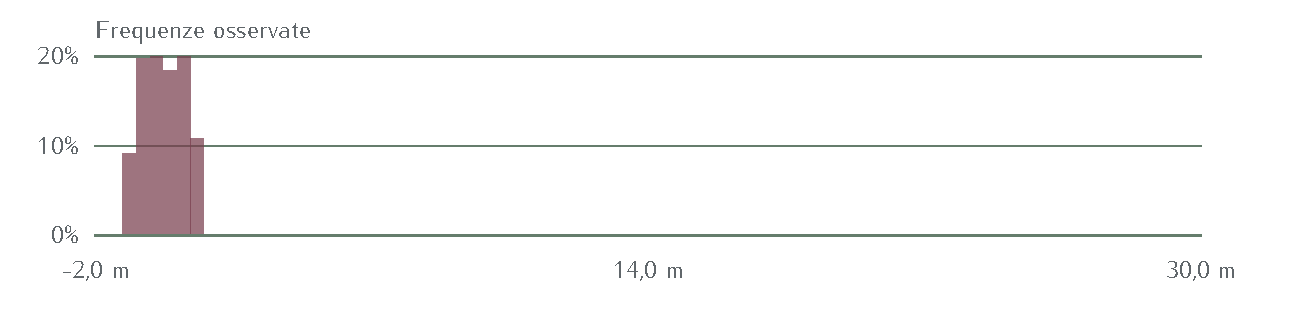
\includegraphics[width=\linewidth,height=94mm,keepaspectratio]{figure/f473b887929b75220.pdf}\FigureCaption{Istogramma di 5000 posizioni al tempo 0,0}\end{FigureBlock}


\BookHeading{Due moti e la loro rappresentazione nel tempo}
Le due righe superiori mostrano \(A\) in verde e \(B\) in corallo sullo stesso asse delle posizioni. Il cerchio vuoto indica il punto di partenza; il punto pieno la posizione all'istante attuale. Il segmento che parte dal punto indica il verso del moto e cresce con la velocità.\par

Nel grafico sotto, l'asse orizzontale misura il tempo e quello verticale la posizione in metri. Ogni punto della retta descrive quindi una posizione a un certo istante, non una curva percorsa nello spazio. La fascia azzurra indica l'intervallo consentito dall'incertezza sulla velocità di \(A\). Cambiare un dato iniziale riporta l'esperimento al tempo zero.\par


Dopo 0,0 s, \(A\) si trova a 0,0 m e \(B\) a 0,0 m. La stessa posizione iniziale è compatibile con moti diversi. L'incertezza sulla velocità amplia l'intervallo delle posizioni previste nel tempo.\par


\BookHeading{Quali dati servono per prevedere il moto?}
\BookHeading{Dalla velocità alla posizione}
Il modello considera un moto lungo una retta, a velocità costante. Se una particella parte da 2 m e percorre 3 m ogni secondo, dopo 4 s avrà compiuto uno spostamento di 3 \(\times\) 4 \(=\) 12 m. La posizione finale è dunque 2 + 12 \(=\) 14 m. Per una velocità negativa lo spostamento si sottrae alla posizione di partenza: il segno distingue i due versi del moto.\par

Nel grafico inferiore del primo disegno il tempo cresce verso destra e la posizione si legge in verticale. Una retta più inclinata indica un cambiamento più rapido della posizione. Le rette di \(A\) e \(B\) iniziano nello stesso punto; se le velocità sono uguali, coincidono per tutta la durata dell'esperimento.\par

\BookHeading{Un intervallo di dati produce un intervallo di previsioni}
Impostiamo per \(A\) una velocità di 3 m/s con incertezza di 0,5 m/s. Consideriamo così possibili tutte le velocità fra 2,5 e 3,5 m/s. Partendo da 0, dopo 4 s le posizioni estreme saranno 2,5 \(\times\) 4 \(=\) 10 m e 3,5 \(\times\) 4 \(=\) 14 m. La fascia colorata comprende le posizioni fra questi estremi. Con il passare del tempo si allarga, perché piccole differenze di velocità si accumulano nello spostamento.\par

L'istogramma aggiunge molte preparazioni indipendenti. Il programma sceglie una posizione e una velocità entro gli intervalli indicati, senza favorire alcuna parte di ciascun intervallo. Conta poi quante particelle arrivano in ogni tratto della retta. Questo criterio di scelta è un'ipotesi ulteriore: conoscere soltanto gli estremi possibili non stabilisce quanto spesso compaia ciascun valore.\par

Confronta una raccolta di 1.000 preparazioni con una di 20.000, lasciando fisse le incertezze. La forma delle barre diventa più regolare, ma l'intervallo delle posizioni possibili resta lo stesso. Un numero maggiore di simulazioni descrive meglio l'incertezza assegnata; per restringerla occorrono dati iniziali più precisi.\par


Il modello e le sue condizioni\par

Le particelle si muovono lungo una retta senza cambiare velocità e senza interagire. La posizione finale si ottiene aggiungendo alla posizione iniziale lo spostamento: velocità moltiplicata per tempo. La fascia comprende tutte le posizioni compatibili con l'intervallo di velocità; da sola non assegna frequenze ai valori al suo interno. Il tempo è espresso in secondi e le posizioni in metri.\par


% Authoritative exercise source. Preserve all derivations and diagrams.

\ExerciseStart{G1.01}{Prevedere due moti dagli stessi dati di posizione}{Guida esplicita}

\BookHeading{Problema, dati e obiettivo}

Due corpi hanno posizione iniziale \(x_0=2\,\mathrm m\). Nel moto A la velocità costante è \(v_A=3\,\mathrm{m/s}\); nel moto B è \(v_B=-1\,\mathrm{m/s}\). Calcolare le posizioni a \(t=0,1,2\,\mathrm s\) e stabilire quale informazione distingua le due previsioni.

\ExTheory{\ExRef{c1-moto}{1.01}}{Nel moto rettilineo uniforme \(x(t)=x_0+vt\). La velocità è la pendenza \(\Delta x/\Delta t\) del grafico posizione-tempo. L’ipotesi di velocità costante esclude accelerazioni durante l’intervallo considerato.}

\ExPrediction{Entrambe le rette attraversano \((0,2)\). Una velocità negativa produce una retta decrescente. Disegnare prima le direzioni delle due rette, poi collocare i punti numerici.}

\ExFigure{\begin{tikzpicture}[>=Stealth,exlabel]
\draw[exaxis] (0,0)--(4,0) node[right] {$t$ (s)};\draw[exaxis] (0,-.2)--(0,3.2) node[above] {$x$ (m)};\fill[Accent] (0,.7) circle(2pt);\node[left] at (0,.7) {$2$};\draw[exvec] (0,.7)--(1.5,2);\draw[exother] (0,.7)--(1.5,.25);
\end{tikzpicture}}{Previsione qualitativa nel piano tempo-posizione: un punto iniziale comune e pendenze differenti.}


\begin{ExTasks}

\item Sostituire i dati nelle due leggi orarie.

\item Calcolare separatamente le posizioni a un secondo.

\item Calcolare le posizioni a due secondi.

\item Ricavare le pendenze dai punti ottenuti.

\item Calcolare la distanza fra i corpi a due secondi e interpretare il ruolo della velocità iniziale.

\end{ExTasks}

\ExSolution

\ExStep{Scrivere le leggi orarie}

Con \(t\) espresso in secondi e \(x\) in metri,
\ExEq{x_A(t)&=2+3t,\qquad x_B(t)=2-t.}
Per \(t=0\) si ottengono \(2+3\cdot0=2\) e \(2-0=2\). Il dato di posizione iniziale è comune.

\ExStep{Calcolare il primo istante}

A un secondo il prodotto \(vt\) è uno spostamento:
\ExEq{x_A(1)&=2+3\cdot1=5\,\mathrm m,\\x_B(1)&=2-1\cdot1=1\,\mathrm m.}
Le unità soddisfano \((\mathrm{m/s})\mathrm s=\mathrm m\).

\ExStep{Calcolare il secondo istante}

A due secondi,
\ExEq{x_A(2)&=2+3\cdot2=8\,\mathrm m,\\x_B(2)&=2-1\cdot2=0\,\mathrm m.}
Nel moto B si raggiunge l’origine; la velocità rimane negativa anche in quel punto.

\ExStep{Verificare le pendenze}

Dai punti iniziale e finale si ricava
\ExEq{\frac{x_A(2)-x_A(0)}{2-0}&=\frac{8-2}{2}=3\,\mathrm{m/s},\\
\frac{x_B(2)-x_B(0)}{2-0}&=\frac{0-2}{2}=-1\,\mathrm{m/s}.}
Il grafico e la formula restituiscono le stesse velocità.

\ExStep{Confrontare le previsioni}

La separazione finale è \(|8-0|=8\,\mathrm m\). In generale \(x_A(t)-x_B(t)=(3-(-1))t=4t\). La sola posizione a \(t=0\) ammette entrambe le evoluzioni; assegnare anche la velocità determina la previsione entro il modello.

\par\noindent\begin{minipage}{\linewidth}
\ExFigure{\begin{tikzpicture}[>=Stealth,exlabel]
\draw[exaxis] (0,0)--(4.7,0) node[right] {$t$ (s)};\draw[exaxis] (0,-.2)--(0,3.6) node[above] {$x$ (m)};\draw[exvec] (0,.8)--(4,3.2) node[right] {$A$};\draw[exother] (0,.8)--(4,0) node[below right] {$B$};\foreach \x/\y/\txt in {0/.8/2,2/2/5,4/3.2/8,2/.4/1}{\fill (\x,\y) circle(1.5pt);\node[above left] at (\x,\y) {$\txt$};}\foreach \x/\t in {2/1,4/2}{\node[below] at (\x,0) {$\t$};}
\end{tikzpicture}}{Dati calcolati. Le scale dei due assi sono differenti e le pendenze numeriche si leggono nelle rispettive unità.}


\ExInterpret{La geometria delle rette rende visibile la dipendenza dai dati iniziali. Due descrizioni con la stessa posizione possono prevedere evoluzioni diverse quando differiscono le velocità.}

\ExLab{Nella sezione 1.01 impostare posizione iniziale 2, velocità A 3 e velocità B \(-1\), con incertezza nulla. Avanzare mediante quattro passi di \(0{,}5\,\mathrm s\) e controllare le due posizioni finali. Cambiare soltanto \(v_B\) in 3: le traiettorie devono coincidere.}


\end{minipage}

% Authoritative exercise source. Preserve all derivations and diagrams.

\ExerciseStart{G1.02}{Propagare un'incertezza sulla velocità}{Guida esplicita}

\BookHeading{Problema, dati e obiettivo}

La posizione iniziale è nota: \(x_0=1\,\mathrm m\). La velocità costante appartiene all’intervallo \([1{,}8;2{,}2]\,\mathrm{m/s}\). Determinare gli intervalli di posizione a 5 e 10 secondi e separare il valore centrale dall’incertezza.

\ExTheory{\ExRef{c1-moto}{1.01}}{Per \(t\geq0\), la funzione \(x_0+vt\) è crescente rispetto a \(v\). Se \(v=\bar v\pm\delta v\), allora \(x(t)=x_0+\bar vt\pm t\delta v\). Un intervallo di valori possibili non assegna da solo una distribuzione di probabilità.}

\ExPrediction{Le rette delle velocità estreme delimitano un cuneo. La larghezza cresce con il tempo mentre il punto iniziale resta comune.}

\ExFigure{\begin{tikzpicture}[>=Stealth,exlabel]
\node[exbox] (n0) at (0.0,0.0) {$x_0=1$};\node[exbox] (n1) at (3.6,0.0) {$v\in[1{,}8;2{,}2]$};\draw[exother] (n0)--(n1);\node[exbox] (n2) at (7.2,0.0) {$x=1+vt$};\draw[exother] (n1)--(n2);
\end{tikzpicture}}{Dati dell’esperimento: una posizione nota e un insieme di velocità ammesse.}


\begin{ExTasks}

\item Ricavare velocità centrale e semilarghezza.

\item Propagare l’estremo inferiore a 5 secondi.

\item Propagare l’estremo superiore e trovare il centro.

\item Ripetere a 10 secondi.

\item Confrontare le due larghezze e indicare che cosa occorrerebbe per assegnare probabilità.

\end{ExTasks}

\ExSolution

\ExStep{Descrivere l’intervallo iniziale}

\ExEq{\bar v&=(1{,}8+2{,}2)/2=2,\\\delta v&=(2{,}2-1{,}8)/2=0{,}2\,\mathrm{m/s}.}
La larghezza totale delle velocità è \(0{,}4\,\mathrm{m/s}\).

\ExStep{Propagare a cinque secondi}

\ExEq{x_{\min}(5)&=1+1{,}8\cdot5=1+9=10\,\mathrm m,\\x_{\max}(5)&=1+2{,}2\cdot5=1+11=12\,\mathrm m.}
Ogni velocità ammessa produce una posizione fra questi estremi.

\ExStep{Verificare centro e semilarghezza}

\ExEq{\bar x(5)&=1+2\cdot5=11\,\mathrm m,\\\delta x(5)&=5\cdot0{,}2=1\,\mathrm m.}
Il risultato \(11\pm1\) ricostruisce \([10;12]\).

\ExStep{Raddoppiare il tempo}

\ExEq{x_{\min}(10)&=1+1{,}8\cdot10=19\,\mathrm m,\\x_{\max}(10)&=1+2{,}2\cdot10=23\,\mathrm m,\\\bar x(10)&=21\,\mathrm m,\qquad\delta x(10)=2\,\mathrm m.}
La larghezza passa da \(12-10=2\) a \(23-19=4\,\mathrm m\).

\ExStep{Interpretare l’insieme delle previsioni}

In generale \(w(t)=x_{\max}-x_{\min}=(2{,}2-1{,}8)t=0{,}4t\). Ogni traiettoria resta deterministica una volta fissata la velocità. Per predire quanti corpi occupino ciascun intervallo occorrerebbe specificare anche come le velocità siano distribuite nell’insieme iniziale.

\par\noindent\begin{minipage}{\linewidth}
\ExFigure{\begin{tikzpicture}[>=Stealth,exlabel]
\draw[exaxis] (0,0)--(5,0) node[right] {$t$ (s)};\draw[exaxis] (0,0)--(0,3.5) node[above] {$x$ (m)};\fill[Secondary!15] (0,.13)--(4,2.99)--(4,2.47)--cycle;\draw[Secondary] (0,.13)--(4,2.99) node[right] {$23$};\draw[Secondary] (0,.13)--(4,2.47) node[right] {$19$};\draw[Accent,dashed] (0,.13)--(4,2.73);\draw[Ink!40] (2,1.3)--(2,1.56);\node[below] at (2,0) {$5$};\node[below] at (4,0) {$10$};
\end{tikzpicture}}{Inviluppo delle traiettorie; le sezioni verticali sono gli intervalli di posizione ai tempi scelti.}


\ExInterpret{L’allargamento deriva dalla propagazione di un’incertezza iniziale. La geometria del cuneo esprime la legge lineare \(\delta x=t\delta v\).}

\ExLab{Nella sezione 1.01 scegliere posizione iniziale 1, velocità A 2 e incertezza sulla velocità A \(0{,}2\). Confrontare gli estremi a 5 e 10 secondi. Nella distribuzione dei campioni distinguere il supporto teorico dai conteggi finiti.}


\end{minipage}

\Needspace{.43\textheight}
\section{Reversibilità e inversione di Loschmidt}
\phantomsection\label{c1-loschmidt}

{\sffamily\small\color{Ink!70} Riferimento alle slide: p. 50.\par}

{\sffamily\small\color{Ink!70} Laboratorio locale: \nolinkurl{index.html#capitolo-1/loschmidt}\par}

Il gas viene preparato nella metà sinistra del recipiente e lasciato espandere. L'esperimento si ferma prima di invertire le velocità. Da quella stessa configurazione partono due ritorni: uno usa tutti i dati disponibili, l'altro introduce l'imprecisione scelta. Il confronto rende osservabile il ruolo dell'informazione necessaria a ricostruire il moto.\par


\BookHeading{Preparazione e significato dei comandi}

\BookHeading{Preparazione e tempi}
Numero di particelle\par

Ogni punto è una particella simulata. Cambiare il numero prepara un nuovo esperimento; il moto precedente viene azzerato.\par

Durata minima di ciascuna fase\par

È il tempo di visione, misurato con un orologio reale. Espansione e ritorno hanno la stessa durata impostata; il calcolo può richiedere più tempo su un dispositivo lento.\par

Tempo simulato prima dell'inversione\par

Stabilisce quanto evolve fisicamente il gas prima del cambio di verso. Le unità di tempo, indicate con u.t., appartengono al modello e non sono secondi reali.\par

Interazione fra particelle\par

Nella prima opzione, particelle vicine si respingono e modificano le rispettive velocità. Nella seconda si attraversano senza influenzarsi; rimangono i rimbalzi sulle pareti.\par

La repulsione agisce entro 3,8 u.l., con la stessa distanza per tutte le popolazioni. Aumentare il numero di particelle nello stesso recipiente aumenta la densità e può modificare la frequenza degli incontri.\par

\BookHeading{Precisione dell'inversione}
Origine dell'imprecisione\par

La registrazione incompleta conserva una direzione arrotondata. L'errore d'inversione parte invece dalla direzione nota e la altera nel momento in cui si cambia il verso del moto.\par

Passo della registrazione angolare\par

Con un passo di \(5{}^{\circ} \), il programma conserva soltanto direzioni multiple di \(5{}^{\circ} \): per esempio \(12{}^{\circ} \) diventa \(10{}^{\circ} \). L'inversione usa questo dato arrotondato. Il valore 0 mantiene la direzione completa.\par

Velocità interessate\par

Sceglie a quante particelle applicare l'imprecisione. Tutte le altre velocità vengono invertite accuratamente.\par

Con \(0{}^{\circ} \) i due ritorni coincidono. Un passo di registrazione di \(1{}^{\circ} \) conserva soltanto il grado più vicino alla direzione misurata. I moduli delle velocità rimangono invariati entro la precisione numerica.\par

\BookHeading{Lettura del confronto}
\guillemotleft{}Particelle\guillemotright{} mostra i punti; \guillemotleft{}Densità\guillemotright{} raggruppa i conteggi in regioni; \guillemotleft{}Velocità\guillemotright{} aggiunge segmenti dal punto verso la direzione del moto. Cambia il disegno, mentre l'evoluzione resta la stessa.\par

L'espansione si arresta prima dell'inversione. Dopo il confronto, la stessa configurazione può essere riutilizzata con un errore diverso. I risultati restano visibili fino a una nuova azione.\par


\BookHeading{Figure della configurazione iniziale}
\begin{FigureBlock}\centering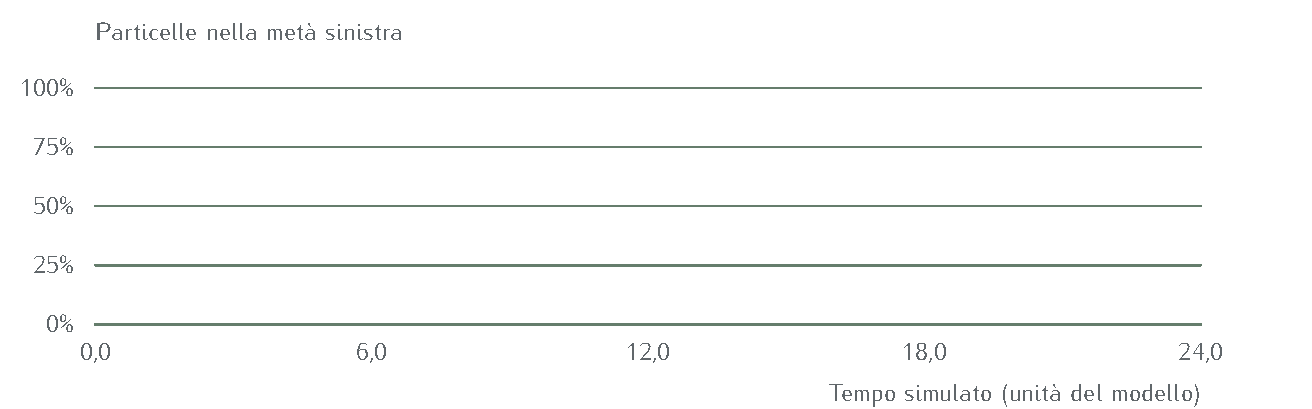
\includegraphics[width=\linewidth,height=94mm,keepaspectratio]{figure/f077e3ac633cde7f8.pdf}\FigureCaption{Quanta parte del gas ritorna nella regione iniziale?. Tempo simulato (unità del modello); Particelle nella metà sinistra}\end{FigureBlock}


\BookHeading{Due criteri per valutare il ritorno}
La prima percentuale conta quante particelle occupano la metà sinistra, dove il gas era stato preparato. La seconda confronta ogni particella con la propria posizione iniziale e conta quelle che distano al massimo 2 unità di lunghezza dal punto di partenza. Per confronto, la larghezza del recipiente è 720 unità. I due criteri distinguono il ritorno nella regione iniziale dal recupero delle posizioni individuali.\par

Il confronto conclusivo va letto quando il tempo di ritorno uguaglia quello di espansione. Durante il tragitto le particelle stanno ancora ripercorrendo il moto: una distanza dalla posizione iniziale non è, da sola, un errore. Il recipiente con particelle verdi fornisce il riferimento; quello con particelle corallo mostra il risultato dell'imprecisione scelta.\par

Il tratteggio verticale divide il recipiente per il conteggio e non è una parete. Invertire una velocità significa mantenere quanto rapidamente la particella si muove e cambiarne il verso. Le posizioni nel momento dell'inversione restano identiche nei due ritorni.\par


\BookHeading{Preparazione iniziale}
Le 5000 particelle occupano la metà sinistra del recipiente. L'espansione durerà almeno 45 secondi e si fermerà prima dell'inversione.\par


All'inizio tutte le particelle si trovano nella metà sinistra. Durante l'espansione il loro numero in questa regione cambia. Gli incontri fra particelle modificano le velocità. La descrizione microscopica conserva posizioni e velocità di ciascuna particella.\par


Il modello e le sue condizioni\par

Le particelle si respingono quando si avvicinano e rimbalzano sulle pareti senza perdere energia. Gli incontri hanno una durata finita: sono descritti da una forza di repulsione, non dall'urto istantaneo fra palline rigide. Il disegno ingrandisce i punti per renderli visibili. Il recipiente è largo 720 e alto 340 unità di lunghezza; queste unità sono indicate con u.l.\par

Il calcolo conserva posizioni e velocità su una griglia numerica. Ogni passo può essere invertito sulla stessa griglia: questo permette al riferimento di recuperare le posizioni iniziali, con velocità di verso opposto. Il tempo simulato avanza con un passo fisso, indipendente dalla rapidità dell'animazione. La reversibilità del procedimento è distinta dalla sua approssimazione delle equazioni fisiche continue.\par

Al momento dell'inversione viene conservata una sola configurazione. I due ritorni sono ricalcolati applicando le forze, senza riprodurre una registrazione delle traiettorie. Nell'inversione incompleta si arrotondano le direzioni prima di cambiarne il verso; nell'inversione perturbata si devia la direzione dopo il cambio di verso. L'imprecisione viene applicata una sola volta. Le formule e le scelte numeriche sono documentate nel file MODELLI incluso nel pacchetto locale.\par

Il risultato riguarda questo sistema isolato nel modello, con tutte le forze e tutte le particelle sotto controllo. Un ritorno imperfetto mostra l'effetto dell'informazione perduta o del controllo incompleto entro questa dinamica reversibile. Riferimento sul metodo numerico reversibile: Rein e Tamayo, JANUS (2017).\par


% Authoritative exercise source. Preserve all derivations and diagrams.

\ExerciseStart{G1.03}{Invertire un moto e ritrovare la preparazione}{Guida esplicita}

\BookHeading{Problema, dati e obiettivo}

Un corpo libero parte da \(x_0=1\,\mathrm m\) con velocità \(v=2\,\mathrm{m/s}\). Dopo \(T=3\,\mathrm s\) si inverte esattamente la velocità. Determinare la traiettoria di ritorno e l’istante in cui il corpo ritrova la posizione iniziale.

\ExTheory{\ExRef{c1-loschmidt}{1.02}}{La dinamica libera è \(x=x_0+vt\). L’inversione cambia \(v\) in \(-v\) conservando la posizione raggiunta. Conviene usare \(\tau=t-T\) per il tempo trascorso dopo l’inversione.}

\ExPrediction{Il ritorno ripercorre le stesse posizioni in ordine inverso. Nel grafico posizione-tempo le due pendenze hanno segni opposti; nel piano posizione-velocità l’intervento cambia la seconda coordinata.}

\ExFigure{\begin{tikzpicture}[>=Stealth,exlabel]
\node[exbox] (n0) at (0.0,0.0) {$(1,2)$};\node[exbox] (n1) at (3.6,0.0) {$(7,2)$};\draw[exother] (n0)--(n1);\node[exbox] (n2) at (7.2,0.0) {$(7,-2)$};\draw[exother] (n1)--(n2);\node[exbox] (n3) at (0.0,-1.6) {$(1,-2)$};\draw[exother] (n2.south)--++(0,-.4)-|(n3.north);\node[exbox] (n4) at (3.6,-1.6) {$(1,2)$};\draw[exother] (n3)--(n4);
\end{tikzpicture}}{Punti nel piano posizione-velocità. I cambi di segno sono interventi istantanei; gli altri passaggi sono evoluzioni libere.}


\begin{ExTasks}

\item Calcolare la posizione al tempo di inversione.

\item Scrivere la legge usando \(\tau\).

\item Calcolare le posizioni dopo uno e due secondi di ritorno.

\item Risolvere l’equazione di ritorno a \(x_0\).

\item Tradurre il risultato nel tempo totale e distinguere posizione e stato completo.

\end{ExTasks}

\ExSolution

\ExStep{Arrivare al punto di inversione}

\ExEq{x(T)&=1+2\cdot3=7\,\mathrm m.}
La coppia prima dell’intervento è \((x,v)=(7,2)\); immediatamente dopo è \((7,-2)\).

\ExStep{Impostare il ritorno}

\ExEq{x_R(\tau)&=7+(-2)\tau=7-2\tau,\qquad\tau\geq0.}
Il nuovo tempo parte da zero al momento dell’intervento.

\ExStep{Seguire gli istanti intermedi}

\ExEq{x_R(1)&=7-2=5,\qquad x_R(2)=7-4=3.}
All’andata si avevano \(x(2)=5\) e \(x(1)=3\): l’ordine dei punti è invertito.

\ExStep{Trovare il ritorno}

\ExEq{7-2\tau&=1,\quad -2\tau=-6,\quad\tau=3\,\mathrm s,\\t&=T+\tau=3+3=6\,\mathrm s.}
La durata della fase inversa deve uguagliare quella diretta.

\ExStep{Confrontare gli stati}

A \(t=6\) la posizione è 1, mentre la velocità è \(-2\). Si è ritrovata la configurazione spaziale con velocità invertite. Una seconda inversione porta \((1,-2)\) in \((1,2)\), ripristinando anche lo stato iniziale completo.

\par\noindent\begin{minipage}{\linewidth}
\ExFigure{\begin{tikzpicture}[>=Stealth,exlabel]
\draw[exaxis] (0,0)--(6.7,0) node[right] {$t$ (s)};\draw[exaxis] (0,0)--(0,3.3) node[above] {$x$ (m)};\draw[Accent,thick] (0,.4)--(3,2.8);\draw[Secondary,thick] (3,2.8)--(6,.4);\draw[dashed] (3,0)--(3,2.8);\node[below] at (3,0) {$3$};\node[below] at (6,0) {$6$};\node[left] at (0,.4) {$1$};\node[above] at (3,2.8) {$7$};
\end{tikzpicture}}{Traiettoria nel piano tempo-posizione. La cuspide identifica l’inversione, non un salto della posizione.}


\ExInterpret{Questo esempio libero rende esplicita la reversibilità. Nei sistemi a molte particelle il ritorno richiede l’inversione di tutte le velocità pertinenti e una dinamica compatibile con tale simmetria.}

\ExLab{Nella sezione 1.02 scegliere inversione ideale e lasciare alla fase inversa lo stesso tempo della fase diretta. Confrontare il ritorno spaziale delle particelle. Il calcolo qui svolto è il caso libero a una dimensione; urti e pareti della simulazione rendono le traiettorie più articolate.}


\end{minipage}

% Authoritative exercise source. Preserve all derivations and diagrams.

\ExerciseStart{G1.04}{Confrontare ritorno ideale e ritorno perturbato}{Guida esplicita}

\BookHeading{Problema, dati e obiettivo}

Riprendere \(x_0=1\), \(v=2\), \(T=3\), nelle unità SI. All’inversione viene applicata la velocità \(-v+\varepsilon\), con \(\varepsilon=0{,}1\,\mathrm{m/s}\). Calcolare l’errore di ritorno. Estendere il confronto a tre corpi con posizioni iniziali \(-1,0,1\), stessa velocità 2 ed errori rispettivamente \(-0{,}1,0,0{,}1\).

\ExTheory{\ExRef{c1-loschmidt}{1.02}}{L’errore additivo sulla velocità ha unità \(\mathrm{m/s}\). Dopo un tempo inverso \(T\), la posizione finale è \(x_0+vT+(-v+\varepsilon)T=x_0+\varepsilon T\). L’espressione riguarda corpi liberi.}

\ExPrediction{La pendenza del ritorno perturbato è meno negativa per \(\varepsilon>0\); al tempo fissato il corpo si arresta nel calcolo a destra della posizione attesa. Per errori opposti, le posizioni esterne della terna si allontanano simmetricamente.}

\ExFigure{\begin{tikzpicture}[>=Stealth,exlabel]
\node[exbox] (n0) at (0.0,0.0) {$v=2$};\node[exbox] (n1) at (3.6,0.0) {$v_R=-2+\varepsilon$};\draw[exother] (n0)--(n1);\node[exbox] (n2) at (7.2,0.0) {$\Delta x=\varepsilon T$};\draw[exother] (n1)--(n2);
\end{tikzpicture}}{La perturbazione agisce sulla velocità di ritorno e si accumula durante la fase inversa.}


\begin{ExTasks}

\item Calcolare posizione e velocità all’inizio del ritorno.

\item Propagare per tre secondi con la velocità perturbata.

\item Ricavare l’errore simbolico \(\Delta x\).

\item Calcolare le tre posizioni finali della terna.

\item Confrontare centro e ampiezza dell’insieme e discutere il limite \(\varepsilon\to0\).

\end{ExTasks}

\ExSolution

\ExStep{Definire il ritorno perturbato}

\ExEq{x(T)&=1+2\cdot3=7,\qquad v_R=-2+0{,}1=-1{,}9.}
La posizione resta continua durante l’inversione.

\ExStep{Calcolare il punto finale}

\ExEq{x_R(3)&=7-1{,}9\cdot3=7-5{,}7=1{,}3\,\mathrm m,\\\Delta x&=1{,}3-1=0{,}3\,\mathrm m.}
Il ritorno ideale avrebbe dato \(7-2\cdot3=1\).

\ExStep{Generalizzare l’errore}

\ExEq{\Delta x&=x_0+vT-vT+\varepsilon T-x_0=\varepsilon T.}
Con \(T=6\) e lo stesso errore, \(\Delta x=0{,}6\,\mathrm m\). La crescita è lineare in questo modello libero; questo calcolo non stabilisce una legge per sistemi caotici.

\ExStep{Propagare la terna}

Per ciascun corpo si usa \(x_i'=x_i+3\varepsilon_i\):
\ExEq{x_1'&=-1+3(-0{,}1)=-1{,}3,\\x_2'&=0+3\cdot0=0,\\x_3'&=1+3\cdot0{,}1=1{,}3.}
Il centro è \((-1{,}3+0+1{,}3)/3=0\); la larghezza è \(1{,}3-(-1{,}3)=2{,}6\), contro 2 iniziale.

\ExStep{Controllare il limite ideale}

Se \(\varepsilon_i=0\) per tutti i corpi, ciascuna correzione \(3\varepsilon_i\) si annulla. Il centro uguale a zero, da solo, non certifica il ritorno della distribuzione: anche la terna allargata ha centro zero.

\par\noindent\begin{minipage}{\linewidth}
\ExFigure{\begin{tikzpicture}[>=Stealth,exlabel]
\draw[exaxis] (-3.3,0)--(3.6,0) node[right] {$x$ (m)};\foreach \x in {-2,0,2}{\fill[Secondary] (\x,.5) circle(2pt);}\foreach \x in {-2.6,0,2.6}{\fill[Accent] (\x,-.5) circle(2pt);}\node[right] at (3,.5) {inizio};\node[right] at (3,-.5) {ritorno};\draw[->,Ink!40] (-2,.4)--(-2.6,-.4);\draw[->,Ink!40] (2,.4)--(2.6,-.4);\node[below] at (-2.6,-.6) {$-1{,}3$};\node[below] at (2.6,-.6) {$1{,}3$};
\end{tikzpicture}}{Posizioni della terna prima dell’andata e dopo il ritorno perturbato. Le due righe separano i due istanti.}


\ExInterpret{La distribuzione richiede più informazione del suo centro. La precisione dell’inversione e il tempo di ritorno contribuiscono entrambi all’errore finale.}

\ExLab{Nella sezione 1.02 confrontare inversione ideale e inversione perturbata mantenendo uguale il tempo delle due fasi. Osservare particelle e densità, quindi aumentare l’imprecisione di registrazione. Il parametro angolare della simulazione è una perturbazione diversa dall’errore additivo del presente modello: confrontare il meccanismo e la tendenza, senza identificarne i valori numerici.}


\end{minipage}

\Needspace{.43\textheight}
\section{Sovrapposizione e fase relativa}
\phantomsection\label{c1-onde}

{\sffamily\small\color{Ink!70} Riferimento alle slide: p. 92.\par}

{\sffamily\small\color{Ink!70} Laboratorio locale: \nolinkurl{index.html#capitolo-1/onde}\par}

Per simulare un'onda occorre descrivere un'oscillazione in ciascun punto. Le prime due curve rappresentano onde con lo stesso periodo; la terza ne mostra la somma. L'intensità misura l'energia che attraversa una data superficie in un dato tempo: qui è espressa rispetto a quella della sola onda \(A\). Variando il ritardo fra i contributi osserveremo come cambia il segnale risultante.\par


\BookHeading{Preparazione e significato dei comandi}

Ritardo relativo\par

Le due onde hanno lo stesso periodo, cioè impiegano lo stesso tempo a compiere un'oscillazione. Qui si regola lo spostamento di un ciclo rispetto all'altro: \(90{}^{\circ} \) corrisponde a un quarto di periodo, \(180{}^{\circ} \) a mezzo periodo.\par

Questi tre casi permettono di seguire il passaggio dal rinforzo alla cancellazione. Mantieni inizialmente uguali le ampiezze delle due onde.\par

Ampiezza dell'onda \(B\)\par

L'ampiezza è il massimo scostamento dall'equilibrio. L'onda \(A\) ha ampiezza 1: con \(B\) \(=\) 1 i contributi sono uguali, con \(B\) \(=\) 0 rimane soltanto \(A\).\par


\BookHeading{Figure della configurazione iniziale}
\begin{FigureBlock}\centering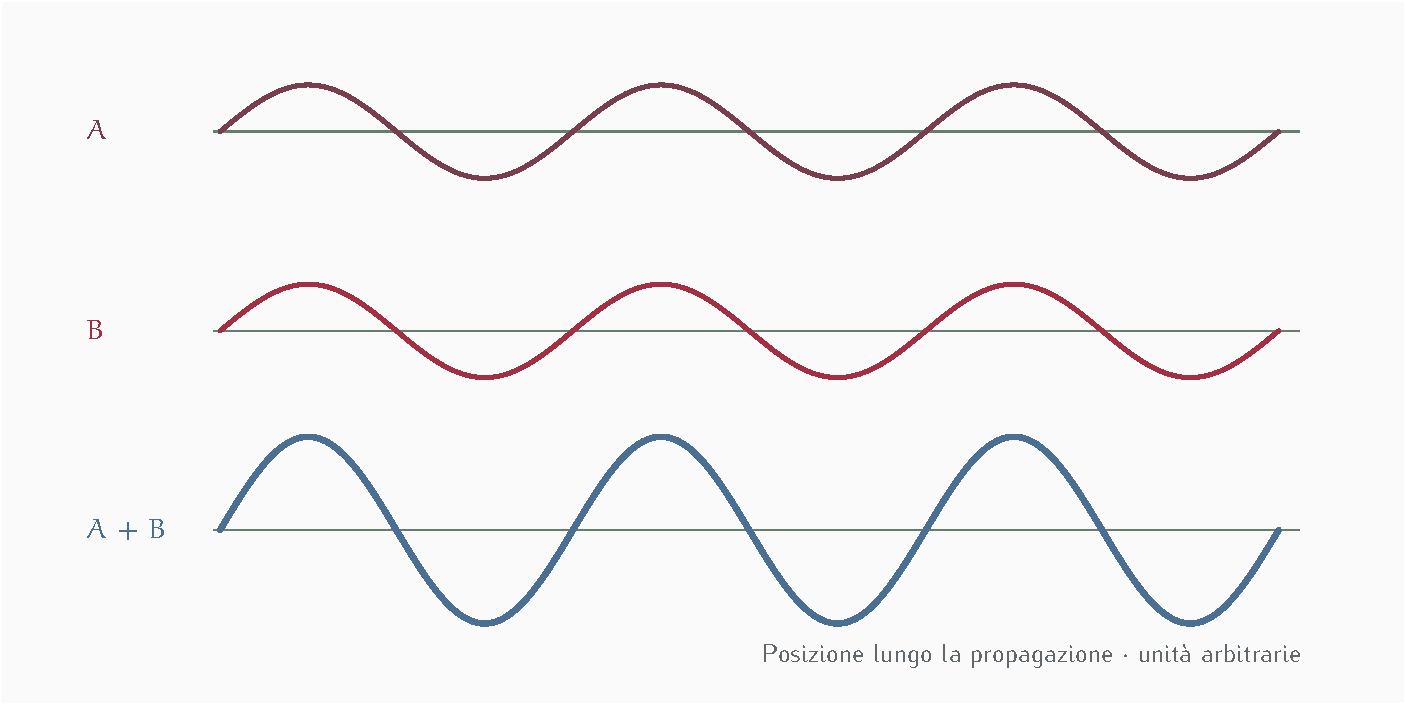
\includegraphics[width=\linewidth,height=94mm,keepaspectratio]{figure/fdf0db99a00c82595.pdf}\FigureCaption{Due onde e la loro somma; ritardo 0 gradi; intensità 4,00}\end{FigureBlock}
\begin{FigureBlock}\centering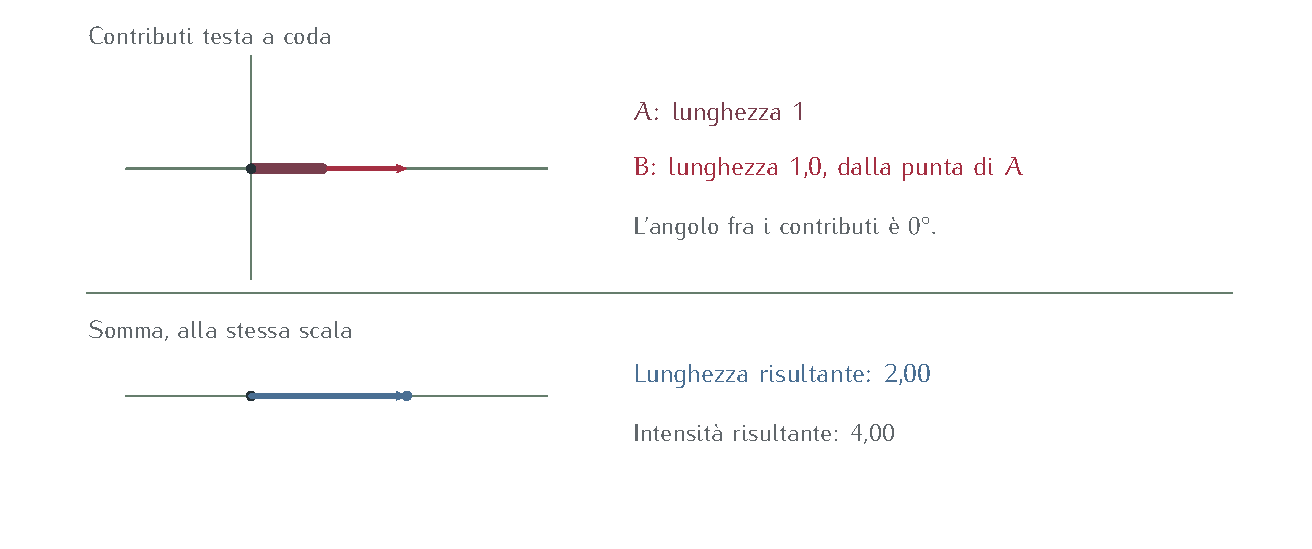
\includegraphics[width=\linewidth,height=94mm,keepaspectratio]{figure/f888eee51b5f36926.pdf}\FigureCaption{Ampiezze sommate testa a coda e risultante alla stessa scala}\end{FigureBlock}
\begin{FigureBlock}\centering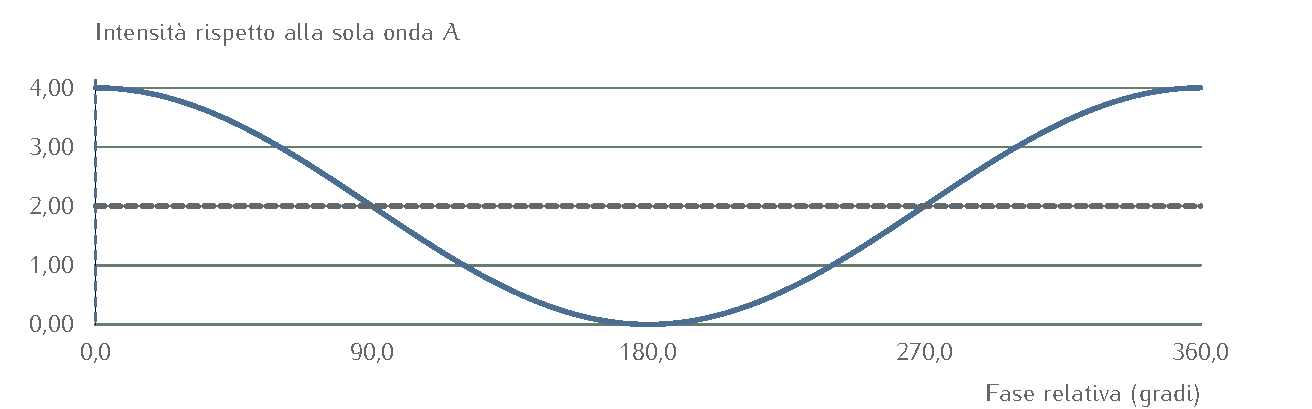
\includegraphics[width=\linewidth,height=94mm,keepaspectratio]{figure/fea07175688d0de07.pdf}\FigureCaption{Dalla fase all'intensità. Fase relativa (gradi); Intensità rispetto alla sola onda \(A\)}\end{FigureBlock}


\BookHeading{Leggere la somma nello stesso istante}
Le tre linee orizzontali segnano il livello di equilibrio. Sopra ogni linea il contributo è positivo, sotto è negativo. In una stessa posizione si somma il valore verde a quello corallo: il risultato forma la curva blu. Le tre curve usano la stessa scala verticale, così il raddoppio e la cancellazione dell'ampiezza sono visibili direttamente.\par

I cicli delle due onde sono allineati: creste e valli coincidono. L'ampiezza \(B\) vale 1,0 rispetto all'ampiezza 1 di \(A\).\par


L'intensità della somma vale 4,00 volte quella della sola onda \(A\). La fase relativa modifica il risultato anche quando le intensità dei singoli contributi rimangono fisse.\par


\BookHeading{Dalle oscillazioni alla figura di interferenza}
\BookHeading{Sommare i contributi nello stesso punto}
In ogni posizione, lo spostamento dell'onda \(A\) si somma a quello dell'onda \(B\) tenendo conto del segno. Se entrambe le onde si trovano a +1 rispetto all'equilibrio, lo spostamento risultante è +2. Se una è a +1 e l'altra a \(- 1\), la somma è 0. La stessa operazione viene ripetuta lungo tutto il profilo e costruisce la terza curva.\par

L'ampiezza è il massimo scostamento dall'equilibrio. Il ritardo relativo stabilisce invece come si dispongono fra loro creste e valli. Con ritardo nullo, due onde uguali raggiungono insieme i massimi e i minimi. Con mezzo ciclo di differenza, a ogni cresta dell'una corrisponde una valle dell'altra: le oscillazioni si compensano in tutte le posizioni.\par

\BookHeading{Un quarto di ciclo nella costruzione geometrica}
La costruzione con le frecce conserva sia l'ampiezza, rappresentata dalla lunghezza, sia la fase, rappresentata dall'orientazione. Si dispone l'inizio della seconda freccia sulla punta della prima; la freccia che va dall'origine alla punta finale rappresenta la somma. \(A\) un quarto di ciclo le due frecce sono perpendicolari. Con entrambe le ampiezze uguali a 1, il quadrato della lunghezza risultante vale 1 + 1 \(=\) 2: questa è l'intensità indicata dal simulatore.\par

\BookHeading{Un confronto che cambia una sola condizione}
Mantenendo uguali le ampiezze, le intensità separate restano fisse anche quando cambia il ritardo. Il programma deve conservare la relazione fra i cicli per prevedere la sovrapposizione; registrare soltanto le due intensità esclude questa informazione.\par

Con l'ampiezza \(B\) ridotta a 0,5 e mezzo ciclo di ritardo, i contributi opposti hanno lunghezze diverse: resta un'ampiezza di 1 \(- \) 0,5 \(=\) 0,5 e un'intensità di 0,5 \(\times\) 0,5 \(=\) 0,25. La cancellazione completa richiede sia l'opposizione di fase sia l'uguaglianza delle ampiezze.\par


Il modello e le sue condizioni\par

Le due onde hanno la stessa forma periodica, lo stesso periodo e la stessa direzione di oscillazione. Il campo risultante è la somma dei campi in ogni punto. L'intensità, calcolata sull'intera oscillazione, è proporzionale al quadrato dell'ampiezza risultante. L'onda \(A\) fornisce l'unità di confronto. L'animazione serve a seguire le oscillazioni; avviarla o fermarla non modifica le intensità previste.\par


% Authoritative exercise source. Preserve all derivations and diagrams.

\ExerciseStart{G1.05}{Sommare due onde con fase assegnata}{Guida esplicita}

\BookHeading{Problema, dati e obiettivo}

Due onde, osservate nello stesso punto, hanno ampiezza unitaria: \(s_A(t)=\cos\omega t\) e \(s_B(t)=\cos(\omega t+\varphi)\). Calcolare l’onda risultante per \(\varphi=0,\pi/2,\pi\) e rappresentare la somma dei contributi nel piano complesso.

\ExTheory{\ExRef{c1-onde}{1.03}}{Il numero \(e^{i\varphi}=\cos\varphi+i\sin\varphi\) rappresenta un segmento unitario orientato di un angolo \(\varphi\). La parte reale di \((1+e^{i\varphi})e^{i\omega t}\) è l’onda osservata. La lunghezza \(|1+e^{i\varphi}|\) ne dà l’ampiezza.}

\ExPrediction{Per contributi concordi prevedere una lunghezza doppia; per contributi opposti una cancellazione. Nel caso di un quarto di ciclo il segmento risultante è la diagonale di un quadrato.}

\ExFigure{\begin{tikzpicture}[>=Stealth,exlabel]
\draw[exaxis] (-0.35,0)--(1.55,0) node[right] {$\operatorname{Re}$};\draw[exaxis] (0,-0.35)--(0,1.55) node[above] {$\operatorname{Im}$};\draw[->,Secondary,line width=1.1pt] (0,0)--(1,0) node[anchor=south west] {$ A $};\draw[->,Accent,line width=1.1pt] (0,0)--(0,1) node[anchor=south west] {$ B $};
\end{tikzpicture}}{Piano dei fasori per un quarto di ciclo: i due contributi hanno uguale lunghezza.}


\begin{ExTasks}

\item Scrivere i due contributi per fase nulla.

\item Costruire la somma per un quarto di ciclo.

\item Calcolare modulo e argomento del risultato \(1+i\).

\item Ripetere per mezzo ciclo.

\item Controllare le tre onde all’istante \(t=0\) e distinguere valore istantaneo e ampiezza.

\end{ExTasks}

\ExSolution

\ExStep{Fase nulla}

\ExEq{e^{i0}&=1,\quad A_0=1+1=2,\\s(t)&=\operatorname{Re}(2e^{i\omega t})=2\cos\omega t.}
L’ampiezza è 2 e la fase della somma è zero.

\ExStep{Un quarto di ciclo}

\ExEq{e^{i\pi/2}&=0+i\cdot1=i,\quad A_{\pi/2}=1+i,\\|A_{\pi/2}|^2&=(1-i)(1+i)=1+i-i-i^2=2.}
Pertanto \(|A_{\pi/2}|=\sqrt2\).

\ExStep{Ricavare la fase della somma}

Le due componenti di \(1+i\) sono positive e uguali. L’angolo è \(\pi/4\), poiché \(\tan(\pi/4)=1\). Quindi
\ExEq{1+i&=\sqrt2\,e^{i\pi/4},\\s(t)&=\sqrt2\cos(\omega t+\pi/4).}

\ExStep{Mezzo ciclo}

\ExEq{e^{i\pi}&=-1,\quad A_\pi=1-1=0,\quad s(t)=0.}
Un vettore nullo non ha un argomento definito: la cancellazione completa elimina l’onda risultante in questo punto.

\ExStep{Verificare un istante}

Per \(t=0\) si hanno rispettivamente \(2\cos0=2\), \(\sqrt2\cos(\pi/4)=1\) e 0. Nel secondo caso il valore istantaneo è 1, mentre l’ampiezza massima è \(\sqrt2\). Il contributo B vale zero in quell’istante, pur avendo ampiezza unitaria.

\par\noindent\begin{minipage}{\linewidth}
\ExFigure{\begin{tikzpicture}[>=Stealth,exlabel]
\draw[exaxis] (-0.35,0)--(1.55,0) node[right] {$\operatorname{Re}$};\draw[exaxis] (0,-0.35)--(0,1.55) node[above] {$\operatorname{Im}$};\draw[->,Secondary,line width=1.1pt] (0,0)--(1,0) node[anchor=south west] {$ 1 $};\draw[->,Secondary,line width=1.1pt] (0,0)--(0,1) node[anchor=south west] {$ i $};\draw[->,Accent,line width=1.1pt] (0,0)--(1,1) node[anchor=south west] {$ 1+i $};\draw[Ink!35,dashed] (1,0)--(1,1)--(0,1);
\end{tikzpicture}}{La diagonale è la somma; i lati tratteggiati completano la costruzione punta-coda.}


\ExInterpret{La fase relativa determina come si combinano le ampiezze. Il piano complesso organizza lunghezze e orientazioni dei contributi, mentre il segnale fisico è la loro parte reale variabile nel tempo.}

\ExLab{Nella sezione 1.03 impostare ampiezza B uguale a quella di A. Confrontare «Insieme», «¼ di ciclo» e «½ ciclo». Seguire sia i fasori sia le onde nel tempo: il massimo del segnale e il suo valore nell’istante mostrato sono grandezze diverse.}


\end{minipage}

% Authoritative exercise source. Preserve all derivations and diagrams.

\ExerciseStart{G1.06}{Dalle ampiezze all'intensità}{Consolidamento}

\BookHeading{Problema, dati e obiettivo}

In un punto del rivelatore arrivano due contributi coerenti di ampiezza reale 2 e 1. Ponendo l’intensità proporzionale al modulo quadro dell’ampiezza, calcolare \(I(\varphi)=|2+e^{i\varphi}|^2\), i valori per \(\varphi=0,\pi/3,\pi/2,\pi\) e la visibilità.

\ExTheory{\ExRef{c1-onde}{1.03}}{Per \(z=a+ib\), \(|z|^2=z^*z=a^2+b^2\). Si definisce visibilità \(V=(I_{\max}-I_{\min})/(I_{\max}+I_{\min})\). Le intensità di ciascun contributo isolato sono \(2^2=4\) e \(1^2=1\), nelle unità relative adottate.}

\ExPrediction{Il contributo più corto può ruotare attorno alla punta di quello maggiore. La distanza dall’origine oscilla fra \(2-1=1\) e \(2+1=3\); prevedere gli estremi dell’intensità prima dello sviluppo algebrico.}

\ExFigure{\begin{tikzpicture}[>=Stealth,exlabel]
\draw[exaxis] (-.4,0)--(3.7,0) node[right] {$\mathrm{Re}$};\draw[exaxis] (0,-1.3)--(0,1.5) node[above] {$\mathrm{Im}$};\draw[Secondary,dashed] (2,0) circle(1);\draw[exvec] (0,0)--(2,0) node[below] {$2$};\draw[exother] (2,0)--(2.5,.866) node[right] {$e^{i\pi/3}$};\draw[Accent!50] (0,0)--(2.5,.866);
\end{tikzpicture}}{Luogo delle punte della somma quando varia la fase. Il cerchio ha raggio uno e centro nel punto 2.}


\begin{ExTasks}

\item Scrivere il coniugato della somma.

\item Svolgere i quattro prodotti distributivi.

\item Raccogliere le due esponenziali in un coseno.

\item Valutare i quattro angoli indicati.

\item Calcolare la visibilità e interpretare il minimo positivo.

\end{ExTasks}

\ExSolution

\ExStep{Costruire il modulo quadro}

\ExEq{I&=(2+e^{-i\varphi})(2+e^{i\varphi})\\&=2\cdot2+2e^{i\varphi}+2e^{-i\varphi}+e^{-i\varphi}e^{i\varphi}\\&=4+2e^{i\varphi}+2e^{-i\varphi}+1.}

\ExStep{Isolare l’interferenza}

\ExEq{e^{i\varphi}+e^{-i\varphi}&=(\cos\varphi+i\sin\varphi)+(\cos\varphi-i\sin\varphi)=2\cos\varphi,\\I(\varphi)&=5+4\cos\varphi.}
Il termine 5 è la somma delle intensità isolate; \(4\cos\varphi\) è il termine incrociato.

\ExStep{Valutare gli angoli}

\ExEq{I(0)&=5+4=9,\\I(\pi/3)&=5+4\cdot\tfrac12=7,\\I(\pi/2)&=5+4\cdot0=5,\\I(\pi)&=5-4=1.}
Nel caso \(\pi/3\), la somma è \(5/2+i\sqrt3/2\), il cui modulo quadro è \(25/4+3/4=7\).

\ExStep{Calcolare la visibilità}

\ExEq{V&=\frac{9-1}{9+1}=\frac8{10}=0{,}8.}
Il minimo resta positivo perché i contributi opposti hanno lunghezze differenti.

\ExStep{Confrontare con ampiezze uguali}

Se il primo contributo fosse anch'esso unitario, \(I=2+2\cos\varphi\), con massimo 4 e minimo 0. La visibilità sarebbe \((4-0)/(4+0)=1\). La fase controlla l’interferenza; il rapporto delle ampiezze ne limita il contrasto.

\par\noindent\begin{minipage}{\linewidth}
\ExFigure{\begin{tikzpicture}[>=Stealth,exlabel]
\draw[exaxis] (-.6,0)--(4.4,0) node[right] {$\varphi$};\draw[exaxis] (-.6,0)--(-.6,3.6) node[above] {$I$};\node[left] at (-.6,3) {$ 10 $};\draw[Ink!15,dashed] (-.6,3)--(3.9000000000000004,3);\filldraw[fill=Accent!25,draw=Accent] (0.0,0) rectangle (0.65,2.7);\node[below] at (0.325,0) {$ 0 $};\node[above] at (0.325,2.7) {$ 9 $};\filldraw[fill=Accent!25,draw=Accent] (1.1,0) rectangle (1.75,2.1);\node[below] at (1.425,0) {$ \pi/3 $};\node[above] at (1.425,2.1) {$ 7 $};\filldraw[fill=Accent!25,draw=Accent] (2.2,0) rectangle (2.85,1.5);\node[below] at (2.5250000000000004,0) {$ \pi/2 $};\node[above] at (2.5250000000000004,1.5) {$ 5 $};\filldraw[fill=Accent!25,draw=Accent] (3.3000000000000003,0) rectangle (3.95,0.3);\node[below] at (3.6250000000000004,0) {$ \pi $};\node[above] at (3.6250000000000004,0.3) {$ 1 $};
\end{tikzpicture}}{Intensità relative nei quattro casi, ottenute dagli stessi contributi.}


\ExInterpret{Il quadrato della somma contiene i prodotti incrociati. Le intensità sono locali: il profilo completo descrive come l’energia si distribuisca sul rivelatore.}

\ExLab{Nella sezione 1.03 scegliere ampiezza B pari a metà di A e variare il ritardo relativo. L’esercizio usa una scala di ampiezza doppia: dividere le intensità calcolate per 4 per confrontarle con una configurazione avente ampiezza A unitaria. La visibilità resta \(0{,}8\).}


\end{minipage}

\Needspace{.43\textheight}
\section{Dai singoli arrivi alla distribuzione}
\phantomsection\label{c1-fenditure}

{\sffamily\small\color{Ink!70} Riferimento alle slide: p. 125.\par}

{\sffamily\small\color{Ink!70} Laboratorio locale: \nolinkurl{index.html#capitolo-1/fenditure}\par}

Ogni evento aggiunge un punto allo schermo. La figura complessiva nasce dall'accumulo di molti arrivi: le regioni più frequentate diventano riconoscibili e possono essere confrontate con la previsione. Cominciamo con una sola apertura, poi apriamo anche la seconda mantenendo fisse le altre condizioni.\par


\BookHeading{Preparazione e significato dei comandi}

\BookHeading{Tre regimi spiegati}
Con una fenditura si osserva il profilo di diffrazione di una singola apertura, dal campo lontano all'impronta di campo vicino. Con due fenditure si può studiare anche il confronto fra i due contributi.\par

Combinazione\par

\guillemotleft{}Con interferenza\guillemotright{} conserva la relazione di fase fra i contributi. \guillemotleft{}Somma dei profili\guillemotright{} somma le probabilità dei due cammini, come nel caso in cui siano distinguibili. Con una sola apertura questa scelta non ha effetto.\par

Larghezza delle fenditure\par

È l'ampiezza fisica a di ciascuna apertura. Un micrometro \((\mu m)\) è un millesimo di millimetro. Nel campo lontano, restringere a allarga il profilo sullo schermo. Nel regime geometrico, invece, la larghezza dell'impronta segue quella dell'apertura, con diffrazione ai bordi. I preset permettono di attraversare questi regimi.\par

Separazione delle fenditure\par

È la distanza d fra i centri delle due aperture. Nel campo lontano determina la distanza approssimata \(\lambda L/d\) fra le frange; nel campo vicino modifica la sovrapposizione dei contributi. Il numero di Fresnel dell'intero apparato usa l'estensione \(D=d+a\).\par

Lunghezza d'onda\par

È la distanza fra due creste successive dell'onda. Un nanometro (nm) è un milionesimo di millimetro; per la luce visibile, lunghezze d'onda diverse corrispondono a colori diversi.\par

Distanza dello schermo\par

Nel campo lontano, aumentare \(L\) dilata la figura; attraversando il regime di Fresnel può cambiare anche la forma del profilo. Nel disegno l'apparato rimane schematico: le distanze fisiche sono quelle impostate nei controlli.\par

Semilarghezza dello schermo\par

Seleziona la finestra visualizzata da \(- s\) a +s millimetri. Le probabilità sono condizionate agli arrivi in questa finestra. La risposta del rivelatore conserva il proprio supporto anche quando comprende punti esterni al ritaglio.\par

Risoluzione del rivelatore\par

È la larghezza dell'intervallo sul quale si media l'intensità in ogni posizione. Il supporto applicato coincide con il valore richiesto; il passo numerico e il metodo di integrazione sono riportati nel profilo e nel CSV. Una risoluzione maggiore può attenuare le frange fini anche con una sorgente coerente.\par

Fase relativa\par

Indica di quanto un contributo è avanti nel ciclo rispetto all'altro. Un giro di \(360{}^{\circ} \) è un ciclo completo; \(90{}^{\circ} \) è un quarto di ciclo e \(180{}^{\circ} \) è mezzo ciclo.\par

Coerenza dei due contributi\par

La coerenza indica quanto viene mantenuta la relazione di fase. Con 1 il modello conserva tutta l'interferenza; con 0 rimane la somma dei profili. I valori intermedi riducono la differenza fra zone chiare e scure.\par


\BookHeading{Figure della configurazione iniziale}
\begin{FigureBlock}\centering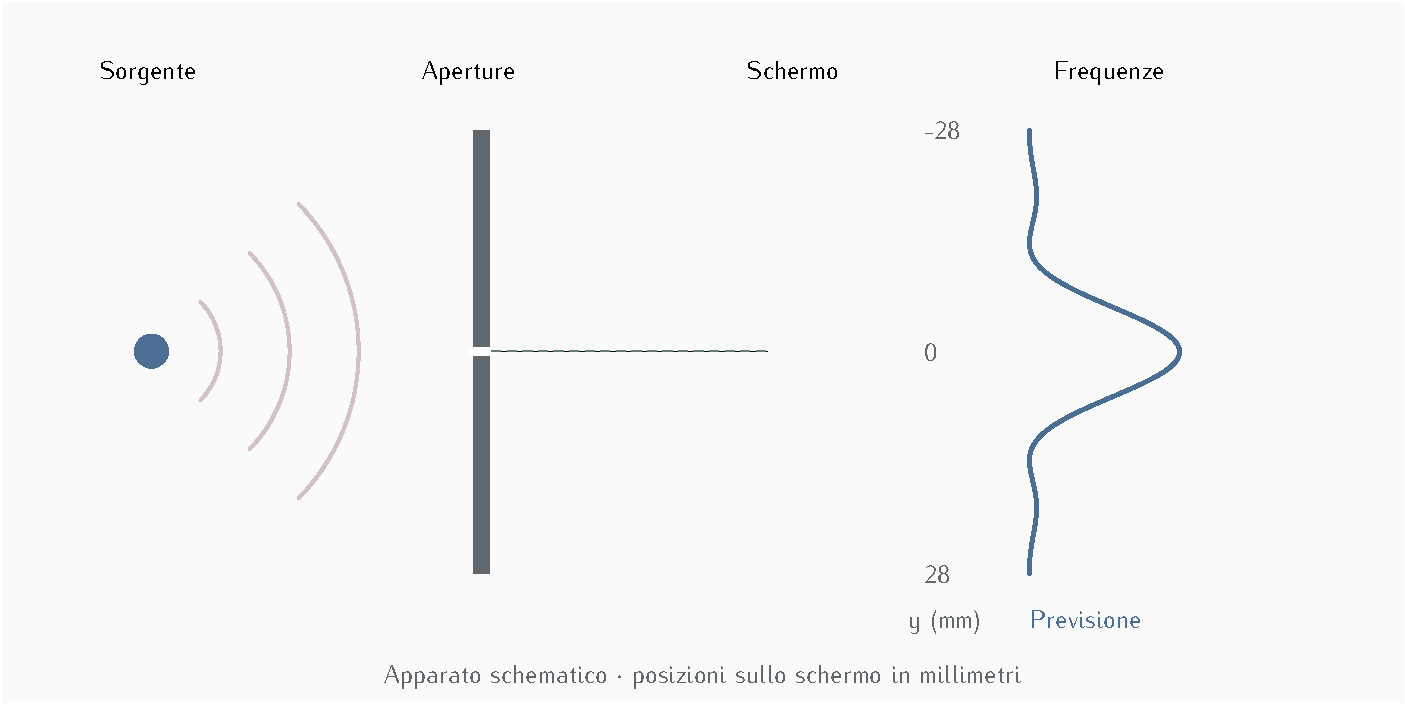
\includegraphics[width=\linewidth,height=94mm,keepaspectratio]{figure/fc6c3031742de02e2.pdf}\FigureCaption{Diffrazione e interferenza: 0 arrivi}\end{FigureBlock}
\begin{FigureBlock}\centering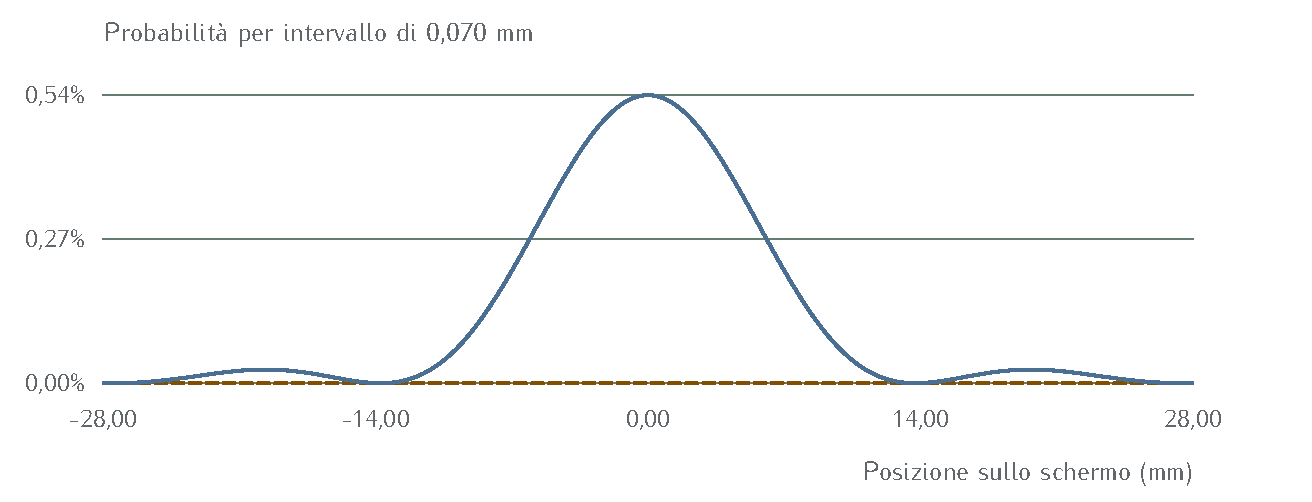
\includegraphics[width=\linewidth,height=94mm,keepaspectratio]{figure/f4283d5c81cc373e9.pdf}\FigureCaption{Confronto risolto fra frequenze e probabilità nelle regioni dello schermo}\end{FigureBlock}


\BookHeading{Lo schermo e le barre contano gli stessi eventi}
L'apparato è schematico: sorgente, aperture e schermo indicano la disposizione dell'esperimento. Sullo schermo, 0 mm è il centro; i valori positivi e negativi distinguono i due lati. La posizione verticale di ogni barra corrisponde alla stessa regione dello schermo. Una barra più lunga significa che vi è arrivata una frazione maggiore degli eventi.\par

Il blu indica la previsione del modello. I punti e le barre verdi si costruiscono invece evento dopo evento. \(A\) raccolta vuota non sono ancora presenti dati da confrontare. Nelle raccolte molto dense il colore dello schermo viene compresso per mantenere visibili sia le regioni deboli sia quelle più popolate: i conteggi esatti restano nelle barre e nel file esportato.\par

Con una sola apertura osserviamo il profilo di diffrazione. La larghezza della fenditura determina il regime: il profilo si allarga nel caso stretto e si avvicina all'impronta geometrica nel caso ampio osservato a risoluzione finita.\par


Sono registrati 0 arrivi. La linea del modello è già visibile; per confrontarla con i dati occorre iniziare la raccolta.\par


\BookHeading{Come leggere la distribuzione degli arrivi}
\BookHeading{Il singolo punto e il profilo della raccolta}
Il punto sullo schermo indica la posizione di una rivelazione. L'istogramma a destra divide lo schermo in piccoli intervalli e conta gli arrivi in ciascuno di essi. Una barra più lunga indica una parte maggiore della raccolta in quella regione. La linea blu mostra le probabilità previste per gli stessi intervalli.\par

Con 100 arrivi possono comparire irregolarità marcate: alcuni intervalli ricevono più eventi di altri anche quando hanno probabilità simili. Proseguendo fino a 10.000 o 100.000 arrivi, il profilo delle frequenze tende a diventare più stabile. Il numero maggiore di eventi migliora la lettura della distribuzione; la forma prevista dipende dall'apparato.\par

\BookHeading{La larghezza del profilo e la distanza fra le frange}
La diffrazione descrive la propagazione dalle aperture anche oltre l'impronta geometrica. Nel campo lontano di una singola fenditura la parte centrale è più popolata, vi sono minimi laterali e restringere l'apertura allarga il profilo. Questa regola richiede \(a^{2}/(\lambda L)\) piccolo: a indica la larghezza intera, \(\lambda \) la lunghezza d'onda e \(L\) la distanza dello schermo. Nel preset intermedio si osserva la transizione di Fresnel; nel preset geometrico l'impronta segue soprattutto la larghezza dell'apertura e rimangono oscillazioni ai bordi, attenuate dalla media del rivelatore.\par

Con due fenditure e una relazione di fase mantenuta, i contributi interferiscono dove si sovrappongono. Nel campo lontano l'inviluppo della singola apertura limita l'estensione delle frange, mentre la separazione d fra i centri ne determina la distanza approssimata \(\lambda L/d\). Per usare insieme queste regole deve essere piccolo \(F_{D}=D^{2}/(\lambda L)\), con \(D=d+a\): il numero \(F_{a}\) della sola fenditura non basta a classificare un apparato con aperture molto distanti. Nel campo vicino il laboratorio calcola direttamente il profilo di Fresnel.\par

La fase relativa cambia le regioni favorite e sfavorite; nel campo lontano questo si legge come uno spostamento delle frange. Ridurre la coerenza attenua il termine di interferenza. Al valore 0 rimane la somma dei profili dei due cammini. La scelta \guillemotleft{}Somma dei profili\guillemotright{} permette di confrontare direttamente questa previsione con quella che conserva l'interferenza. La risoluzione del rivelatore media invece l'intensità su un intervallo spaziale della larghezza dichiarata, senza modificare la coerenza della sorgente.\par

\BookHeading{Che cosa viene confrontato}
Le raccolte sono confrontate a parità di numero di arrivi registrati nella finestra dello schermo. Il laboratorio mostra quindi dove si distribuiscono gli eventi, senza rappresentare l'aumento o la diminuzione della quantità totale di luce trasmessa dalle aperture. Le statistiche distinguono la frazione di flusso nella finestra prima e dopo la media del rivelatore; soltanto in seguito le probabilità visualizzate sono normalizzate al 100\%. La media usa anche il campo esterno alla finestra e conserva la stessa larghezza ai bordi. Quando modifichi l'apparato, la raccolta corrente viene azzerata; puoi conservare prima il profilo per confrontarlo con il successivo. La sua etichetta include la risoluzione, che può differire da quella della nuova raccolta.\par


Il modello e le sue condizioni\par

Il calcolo integra la propagazione scalare di Fresnel di una luce piana, uniforme e monocromatica. È una descrizione paraassiale: apertura, separazione e posizione sullo schermo devono restare piccole rispetto alla distanza. La fenditura è larga rispetto alla lunghezza d'onda. Il numero \(F_{a}=a^{2}/(\lambda L)\), definito con la larghezza intera a, caratterizza ciascuna fenditura. Per l'apparato completo usiamo \(F_{D}=D^{2}/(\lambda L)\), con \(D=a\) per una fenditura e \(D=d+a\) per due, dove d è la separazione dei centri. Il campo lontano dell'intero apparato richiede \(F_{D}\) piccolo; \(F_{a}\) piccolo da solo non basta quando le aperture sono molto separate. La coerenza rimane indipendente dalla larghezza.\par

Le probabilità si riferiscono agli arrivi nella finestra dello schermo, da \(- 28\) a +28 mm. La loro somma nella finestra è il 100\%. Si confrontano così le forme a parità di eventi registrati, senza calcolare il flusso totale trasmesso dall'apparato. Ogni evento contribuisce sia allo schermo sia alle barre. Il confronto resta valido sulla medesima finestra. La risposta del rivelatore è la media rettangolare sulla larghezza richiesta, anche al bordo: il campo è calcolato oltre la finestra prima della media. La linea ambra mostra l'impronta geometrica, mediata sullo stesso supporto. Le oscillazioni fini del campo coerente possono essere risolte diminuendo la larghezza del rivelatore.\par


% Authoritative exercise source. Preserve all derivations and diagrams.

\ExerciseStart{G1.07}{Localizzare i minimi per una fenditura stretta}{Consolidamento}

\BookHeading{Problema, dati e obiettivo}

Una fenditura singola di larghezza \(a=20\,\mu\mathrm m\) è illuminata con luce di lunghezza d’onda \(\lambda=550\,\mathrm{nm}\). Lo schermo è a \(L=1\,\mathrm m\) e mostra \(-70\leq x\leq70\,\mathrm{mm}\). Determinare i primi due minimi sui due lati, la larghezza del massimo centrale e l’intensità relativa a metà strada dal primo minimo. Si assume illuminazione uniforme, propagazione scalare paraxiale e campo lontano.

\ExTheory{\ExRef{c1-fenditure}{1.04}}{Per una singola apertura uniforme, \(I(x)/I(0)=(\sin\beta/\beta)^2\), dove \(\beta=\pi ax/(\lambda L)\). Al centro il rapporto vale uno per continuità. I minimi diversi dal centro soddisfano \(\beta=k\pi\), con \(k\) intero non nullo. Il numero \(F_a=a^2/(\lambda L)\) permette di controllare l’ipotesi di campo lontano.}

\ExPrediction{Prima di calcolare, prevedere la simmetria rispetto a \(x=0\). Se si dimezzasse l’apertura, la scala trasversale \(\lambda L/a\) raddoppierebbe: indicare sulla figura dove ci si attenderebbe il nuovo primo minimo.}

\ExFigure{\begin{tikzpicture}[>=Stealth,exlabel]
\draw[exaxis] (-4.6,0)--(4.8,0) node[right] {$x$ (mm)};
\draw[Accent,very thick] (0,-.4)--(0,.4);
\foreach \x/\lab in {-3.85/-55,-1.925/-27{,}5,0/0,1.925/27{,}5,3.85/55}{\draw (\x,-.08)--(\x,.08);\node[below] at (\x,-.15) {$\lab$};}
\node[above] at (0,.55) {centro dello schermo};
\end{tikzpicture}}{Coordinate fisiche sullo schermo. I segni distinguono i due lati della stessa apertura.}


\begin{ExTasks}

\item Convertire \(a\) e \(\lambda\) in metri e calcolare \(F_a\).

\item Risolvere \(\beta=\pi\) rispetto a \(x\), controllandone l’unità.

\item Calcolare i quattro minimi con \(k=\pm1,\pm2\).

\item Ricavare la distanza fra i primi due minimi ai lati del centro.

\item Calcolare \(I/I(0)\) per \(x=13{,}75\,\mathrm{mm}\) e ripetere la previsione per \(a=10\,\mu\mathrm m\).

\end{ExTasks}

\ExSolution

\ExStep{Controllare il regime}

Le conversioni sono \(a=20\cdot10^{-6}=2\cdot10^{-5}\,\mathrm m\) e \(\lambda=550\cdot10^{-9}=5{,}5\cdot10^{-7}\,\mathrm m\). Pertanto
\ExEq{F_a&=\frac{(2\cdot10^{-5})^2}{(5{,}5\cdot10^{-7})\cdot1}
=\frac{4\cdot10^{-10}}{5{,}5\cdot10^{-7}}
\simeq7{,}27\cdot10^{-4}.}
Il rapporto è adimensionale e molto minore di uno. Il modello di Fraunhofer è quindi appropriato per questa apertura e questa distanza.

\ExStep{Isolare la coordinata del minimo}

Si sostituisce la definizione di \(\beta\):
\ExEq{\frac{\pi ax}{\lambda L}&=k\pi,\\
 ax&=k\lambda L,\qquad x_k=k\frac{\lambda L}{a},\\
\frac{\lambda L}{a}&=\frac{5{,}5\cdot10^{-7}\cdot1}{2\cdot10^{-5}}\,\mathrm m
=0{,}0275\,\mathrm m=27{,}5\,\mathrm{mm}.}
L’unità del rapporto è \(\mathrm m\cdot\mathrm m/\mathrm m=\mathrm m\).

\ExStep{Collocare i minimi}

Per \(k=1\), \(x_1=27{,}5\,\mathrm{mm}\); per \(k=-1\), \(x_{-1}=-27{,}5\,\mathrm{mm}\). Per \(k=2\), \(x_2=2\cdot27{,}5=55\,\mathrm{mm}\); per \(k=-2\), \(x_{-2}=-55\,\mathrm{mm}\). Tutti e quattro appartengono alla finestra dello schermo. Il terzo minimo sarebbe a \(82{,}5\,\mathrm{mm}\), oltre il bordo.

\ExStep{Misurare il massimo centrale}

La sua larghezza, misurata fra i primi zeri, è
\ExEq{w&=x_1-x_{-1}=27{,}5-(-27{,}5)=55\,\mathrm{mm}.}
L’angolo del primo minimo è approssimativamente \(x_1/L=0{,}0275\,\mathrm{rad}\). La piccolezza dell’angolo è coerente con l’approssimazione paraxiale.

\ExStep{Calcolare un punto intermedio}

Per \(x=13{,}75\,\mathrm{mm}=x_1/2\) si ha
\ExEq{\beta&=\pi\frac{x}{x_1}=\frac\pi2,\\
\frac{I(x)}{I(0)}&=\left(\frac{\sin(\pi/2)}{\pi/2}\right)^2
=\left(\frac{1}{\pi/2}\right)^2=\frac4{\pi^2}\simeq0{,}4053.}
Questo rapporto confronta due intensità; una probabilità per un intervallo richiederebbe anche l’integrazione e la normalizzazione sulla finestra.

\ExStep{Variare l’apertura}

Se \(a'=10\,\mu\mathrm m=a/2\), allora
\ExEq{x'_1&=\frac{\lambda L}{a/2}=2\frac{\lambda L}{a}=55\,\mathrm{mm},\\w'&=2x'_1=110\,\mathrm{mm},\qquad F'_a=F_a/4\simeq1{,}82\cdot10^{-4}.}
Il massimo centrale si allarga e la condizione di campo lontano rimane soddisfatta.

\par\noindent\begin{minipage}{\linewidth}
\ExFigure{\begin{tikzpicture}[>=Stealth,exlabel]
\draw[exaxis] (-4.4,0)--(4.6,0) node[right] {$x$ (mm)};\draw[exaxis] (0,0)--(0,2.8) node[above] {$I/I(0)$};
\draw[Accent,thick,domain=-60:60,samples=201] plot ({.07*\x},{2.3*(abs(\x)<.0001 ? 1 : (sin(180*\x/27.5)/(pi*\x/27.5))^2)});
\foreach \x/\lab in {-3.85/-55,-1.925/-27{,}5,1.925/27{,}5,3.85/55}{\fill[Secondary] (\x,0) circle(1.7pt);\node[below] at (\x,0) {$\lab$};}
\draw[Secondary,dashed] (.9625,0)--(.9625,.9322);\node[above right] at (.9625,.9322) {$4/\pi^2$};
\end{tikzpicture}}{Profilo di Fraunhofer per i dati dell’esercizio. La figura mostra intensità relative, senza campionamento casuale.}


\ExInterpret{Gli zeri provengono dalla cancellazione dei contributi dell’apertura. La scala \(\lambda L/a\) collega la geometria dell’apparato alla larghezza del profilo. La formula è stata applicata dopo averne controllato il regime.}

\ExLab{Aprire la sezione 1.04, scegliere una sola fenditura e impostare \(a=20\,\mu\mathrm m\), \(\lambda=550\,\mathrm{nm}\), \(L=1\,\mathrm m\), semilarghezza \(70\,\mathrm{mm}\). Confrontare il profilo teorico di Fresnel con i minimi previsti; mantenere piccola la risoluzione del rivelatore rispetto a \(27{,}5\,\mathrm{mm}\). Dimezzare \(a\) e verificare lo spostamento del primo minimo. Le frequenze di pochi arrivi possono oscillare attorno alla previsione.}


\end{minipage}

% Authoritative exercise source. Preserve all derivations and diagrams.

\ExerciseStart{G1.08}{Attraversare i regimi della diffrazione}{Consolidamento}

\BookHeading{Problema, dati e obiettivo}

Per una singola fenditura mantenere \(\lambda=550\,\mathrm{nm}\), \(L=1\,\mathrm m\), e confrontare \(a=20\,\mu\mathrm m\), \(1\,\mathrm{mm}\), \(8\,\mathrm{mm}\). Nel terzo caso usare una media rettangolare del rivelatore di larghezza \(\delta=0{,}16\,\mathrm{mm}\). Determinare il regime e il riferimento geometrico mediato.

\ExTheory{\ExRef{c1-fenditure}{1.04}}{Il numero \(F_a=a^2/(\lambda L)\) confronta apertura e scala di Fresnel \(\sqrt{\lambda L}\). Il campo lontano richiede \(F_a\ll1\). Nel riferimento geometrico la singola apertura trasmette uniformemente per \(|x|<a/2\). Un rivelatore finito ne media il profilo su un intervallo di larghezza \(\delta\).}

\ExPrediction{Al crescere dell’apertura l’interno dell’immagine geometrica si estende. Le oscillazioni ai bordi hanno una scala relativa sempre più piccola; la media del rivelatore ne attenua quelle che non risolve.}

\ExFigure{\begin{tikzpicture}[>=Stealth,exlabel]
\node[exbox] (n0) at (0.0,0.0) {$F_a\ll1$\ campo lontano};\node[exbox] (n1) at (3.6,0.0) {$F_a\simeq1$\ Fresnel};\draw[exother] (n0)--(n1);\node[exbox] (n2) at (7.2,0.0) {$F_a\gg1$\ interno geometrico};\draw[exother] (n1)--(n2);
\end{tikzpicture}}{Il parametro cambia mantenendo fisse lunghezza d’onda e distanza. La propagazione di Fresnel attraversa tutti e tre i casi.}


\begin{ExTasks}

\item Calcolare \(\lambda L\) e la sua radice.

\item Calcolare i tre numeri di Fresnel.

\item Individuare il caso nel quale usare la formula di campo lontano.

\item Costruire la media geometrica vicino al bordo destro \(b=a/2\).

\item Valutare il riferimento in \(b-\delta/2,b,b+\delta/2\) e descrivere il confronto corretto con Fresnel.

\end{ExTasks}

\ExSolution

\ExStep{Determinare la scala}

\ExEq{\lambda L&=5{,}5\cdot10^{-7}\,\mathrm m^2,\\\sqrt{\lambda L}&\simeq7{,}416\cdot10^{-4}\,\mathrm m=0{,}742\,\mathrm{mm}.}
Questa lunghezza caratterizza la struttura diffrattiva trasversale nel modello paraxiale.

\ExStep{Calcolare i tre regimi}

\ExEq{F_{20\mu m}&=\frac{4\cdot10^{-10}}{5{,}5\cdot10^{-7}}\simeq0{,}000727,\\F_{1mm}&=\frac{10^{-6}}{5{,}5\cdot10^{-7}}\simeq1{,}818,\\F_{8mm}&=\frac{64\cdot10^{-6}}{5{,}5\cdot10^{-7}}\simeq116{,}36.}
Le aperture attraversano campo lontano, regime intermedio e regime prossimo alla geometria nell’interno.

\ExStep{Delimitare la formula dei minimi}

Per \(20\,\mu\mathrm m\), \(x_1=\lambda L/a=27{,}5\,\mathrm{mm}\). Inserire \(8\,\mathrm{mm}\) nella stessa espressione darebbe \(0{,}06875\,\mathrm{mm}\), ma \(F_a\gg1\) invalida l’ipotesi utilizzata per ricavarla. Il profilo in quel regime va propagato con Fresnel.

\ExStep{Mediare il riferimento geometrico}

Per \(a=8\,\mathrm{mm}\), il bordo destro è \(b=4\,\mathrm{mm}\). Vicino a quel bordo, la frazione illuminata dell’intervallo del rivelatore è
\ExEq{G_\delta(x)&=\begin{cases}1&x\leq b-\delta/2,\\(b+\delta/2-x)/\delta&b-\delta/2<x<b+\delta/2,\\0&x\geq b+\delta/2.\end{cases}}
La formula locale vale lontano dal bordo sinistro, che è simmetrico.

\ExStep{Valutare e interpretare la media}

Poiché \(\delta/2=0{,}08\,\mathrm{mm}\),
\ExEq{G_\delta(3{,}92)&=1,\\G_\delta(4)&=(4{,}08-4)/0{,}16=1/2,\\G_\delta(4{,}08)&=0.}
Questi sono valori del riferimento geometrico mediato. Il profilo di Fresnel mediato conserva correzioni ai bordi; l’accordo va valutato alla scala dello schermo, senza imporre uguaglianza punto per punto.

\par\noindent\begin{minipage}{\linewidth}
\ExFigure{\begin{tikzpicture}[>=Stealth,exlabel]
\draw[exaxis] (0,0)--(6.2,0) node[right] {$x$ (mm)};\draw[exaxis] (0,0)--(0,2.8) node[above] {$G_\delta$};\draw[Accent,thick] (0,2)--(2,2)--(4,0)--(5.7,0);\draw[Secondary,dashed] (3,0)--(3,1)--(0,1);\node[left] at (0,2) {$1$};\node[left] at (0,1) {$1/2$};\node[below] at (2,0) {$3{,}92$};\node[below] at (3,-.35) {$4$};\node[below] at (4,0) {$4{,}08$};
\end{tikzpicture}}{Ingrandimento del bordo geometrico dopo la stessa media rettangolare del rivelatore; non è un profilo di Fresnel.}


\ExInterpret{Il limite geometrico riguarda un confronto di scale e di osservabili. Una singola apertura larga può ancora diffrangere ai bordi. Per due aperture occorrerebbe controllare anche l’estensione totale illuminata, oltre alla larghezza di ciascuna.}

\ExLab{Nella sezione 1.04 scegliere «Una» e confrontare i preset «Fenditura stretta», «Regime intermedio» e «Limite geometrico». Nell’ultimo controllare \(a=8\,\mathrm{mm}\) e risoluzione \(0{,}16\,\mathrm{mm}\). Confrontare profilo propagato e ombra geometrica dopo la stessa media. La distribuzione dei conteggi è normalizzata sulla finestra osservata.}


\end{minipage}

\Needspace{.43\textheight}
\section{Polarizzazione, misura e sfera di Bloch}
\phantomsection\label{c1-polarizzazione}

{\sffamily\small\color{Ink!70} Riferimento alle slide: p. 165.\par}

{\sffamily\small\color{Ink!70} Laboratorio locale: \nolinkurl{index.html#capitolo-1/polarizzazione}\par}

Riprendiamo la luce polarizzata usata nella lezione. Il disegno del campo mostra come oscilla la luce; la sfera di Bloch rappresenta la preparazione del qubit; le uscite \(A\) e \(B\) registrano gli esiti della misura. Il laboratorio mette in relazione queste tre descrizioni, mantenendone distinto il significato.\par


\BookHeading{Preparazione e significato dei comandi}

\(H\) indica la polarizzazione orizzontale, \(V\) quella verticale. \(+45{}^{\circ} \) e \(- 45{}^{\circ} \) sono le due diagonali. La diagonale \(+45{}^{\circ} \) ha componenti concordi, quella \(- 45{}^{\circ} \) componenti opposte. Ai poli \(H\) e \(V\) è presente una sola componente. I pulsanti selezionano lo stato completo corrispondente.\par

Orientazione prima dello sfasamento\par

Prima di aggiungere una fase, questo è l'angolo della polarizzazione lineare nel piano del campo. Regola il peso delle componenti orizzontale e verticale. Se poi introduci una fase, la punta del campo può descrivere un'ellisse e non ha più un'unica direzione fissa.\par

Orientazione dell'analizzatore\par

\(A\) \(0{}^{\circ} \) le uscite \(A\) e \(B\) corrispondono rispettivamente a \(H\) e \(V\). \(A\) \(45{}^{\circ} \) corrispondono alle diagonali \(+45{}^{\circ} \) e \(- 45{}^{\circ} \). Ruotare l'analizzatore cambia la domanda posta alla stessa preparazione.\par

Fase aggiunta alla componente \(V\)\par

Cursore \(\cdot\) Fase aggiunta alla componente \(V\)\par

Il comando aggiunge una fase alla polarizzazione lineare scelta. La diagonale \(- 45{}^{\circ} \) parte già con componenti opposte; la lettura dello stato riporta la fase effettiva dopo questa aggiunta.\par


\BookHeading{Figure della configurazione iniziale}
\begin{FigureBlock}\centering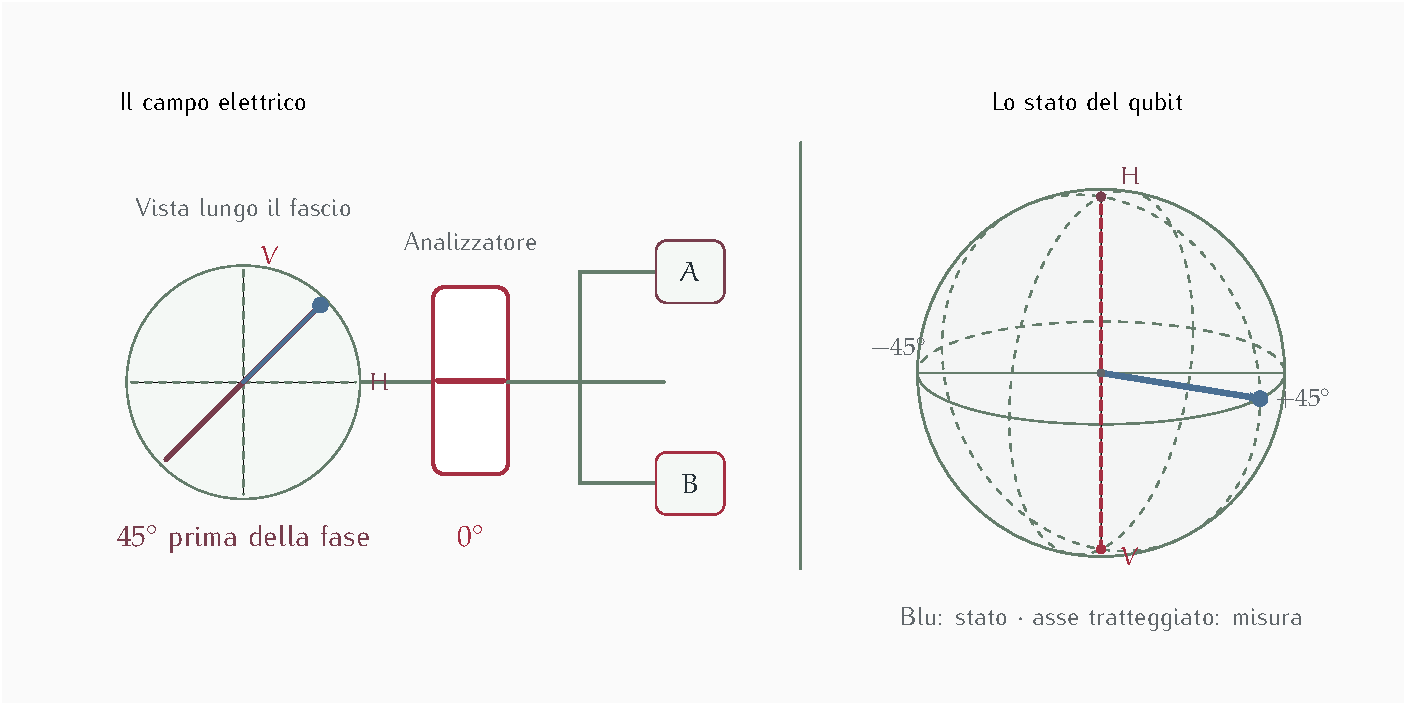
\includegraphics[width=\linewidth,height=94mm,keepaspectratio]{figure/f7065a0e4aca63db0.pdf}\FigureCaption{Polarizzazione 45 gradi; analizzatore 0 gradi; sfera di Bloch dello stato preparato}\end{FigureBlock}
\begin{FigureBlock}\centering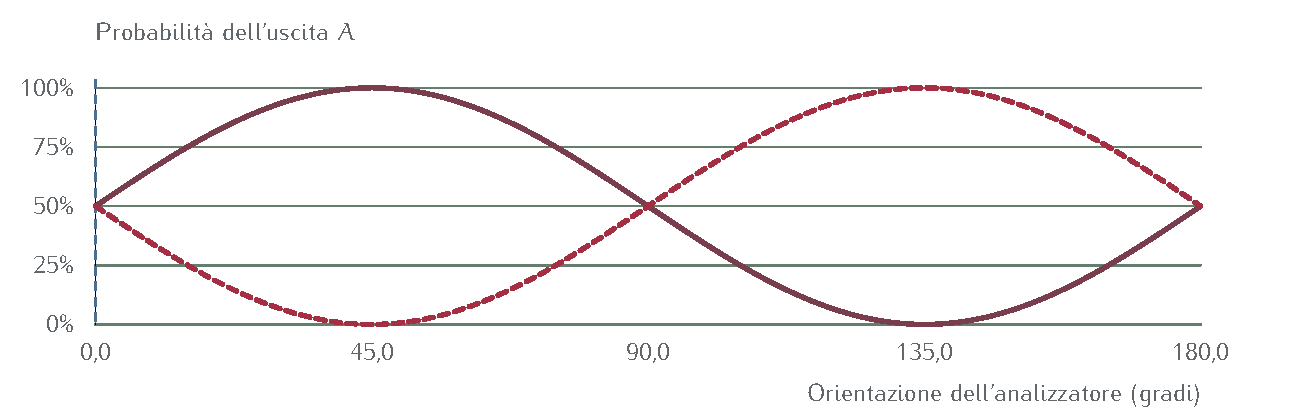
\includegraphics[width=\linewidth,height=94mm,keepaspectratio]{figure/f7b59d219325a6978.pdf}\FigureCaption{La stessa preparazione, tutte le orientazioni di misura. Orientazione dell'analizzatore (gradi); Probabilità dell'uscita \(A\)}\end{FigureBlock}


\BookHeading{Il campo, la preparazione e le due uscite}
Il segmento o l'ellisse a sinistra descrive il movimento della punta del campo elettrico durante un ciclo, guardando il fascio lungo la propagazione. La figura resta in un piano perpendicolare al fascio. L'analizzatore separa due polarizzazioni perpendicolari: \(A\) segue l'orientazione scelta, \(B\) quella a \(90{}^{\circ} \) rispetto ad \(A\).\par

Sulla sfera il punto blu rappresenta la preparazione; l'asse tratteggiato indica la misura. Sono due rappresentazioni diverse: il punto sulla sfera non oscilla insieme al campo. Con l'analizzatore a \(0{}^{\circ} \), i poli \(H\) e \(V\) danno uscite certe, mentre ogni punto dell'equatore dà 50\% e 50\%.\par

Con le impostazioni attuali, il modello prevede 50,0\% in \(A\) e 50,0\% in \(B\). Il campo è lineare: la sua punta percorre il segmento disegnato. Ogni prova registra un solo evento; le percentuali si stimano ripetendo la preparazione.\par


Con l'analizzatore a \(0{}^{\circ} \), la probabilità dell'uscita \(A\) è 50,0\%. Quando entrambe le componenti sono presenti, la fase relativa può modificare la figura del campo e il punto sulla sfera. Una preparazione circolare assegna 50/50 a ogni analizzatore lineare.\par


\BookHeading{Dalla polarizzazione alla scelta della misura}
\BookHeading{Due componenti dello stesso campo}
Guardiamo il fascio lungo la direzione di propagazione. Una polarizzazione \(H\) oscilla orizzontalmente, una polarizzazione \(V\) verticalmente. Nella diagonale a \(+45{}^{\circ} \) il campo ha una componente orizzontale e una verticale di uguale ampiezza, che oscillano insieme. Sono componenti dello stesso campo elettrico.\par

\guillemotleft{}Anima il campo\guillemotright{} segue la punta del vettore lungo le posizioni raggiunte durante un'oscillazione. Per una polarizzazione lineare si ottiene un segmento. Se le due componenti acquistano uno sfasamento, la punta può percorrere un'ellisse; con ampiezze uguali e un quarto di ciclo di differenza percorre un cerchio. Le figure descrivono l'oscillazione del campo di un fascio classico, non il tragitto di un pacchetto di luce nello spazio.\par

\BookHeading{Misurare un pacchetto alla volta}
Con l'analizzatore a \(0{}^{\circ} \), l'uscita \(A\) corrisponde alla polarizzazione \(H\) e l'uscita \(B\) alla polarizzazione \(V\). La preparazione \(H\) conduce sempre ad \(A\) nel modello ideale; la preparazione \(V\) conduce sempre a \(B\). La diagonale a \(+45{}^{\circ} \) assegna invece uguale probabilità ai due esiti.\par

Ogni prova prepara un nuovo pacchetto e registra un solo esito. Su molte prove con la diagonale ci aspettiamo circa metà degli arrivi in \(A\) e metà in \(B\). La scomposizione del campo non significa che ciascun pacchetto sia registrato per metà in ogni uscita. Il 50\% descrive la probabilità dei singoli esiti e il comportamento di una raccolta numerosa.\par

\BookHeading{La stessa ripartizione può provenire da preparazioni diverse}
Prepara prima \(+45{}^{\circ} \) e poi \(- 45{}^{\circ} \), lasciando l'analizzatore a \(0{}^{\circ} \). Entrambe le preparazioni danno probabilità 50\% e 50\%. Sulla sfera occupano però due punti opposti dell'equatore. La stessa altezza rispetto all'asse H/V spiega l'uguaglianza delle probabilità in quella misura; la diversa posizione conserva la differenza fra gli stati.\par

Ruota ora l'analizzatore a \(45{}^{\circ} \). L'uscita \(A\) legge la diagonale \(+45{}^{\circ} \) e \(B\) la diagonale perpendicolare \(- 45{}^{\circ} \). La prima preparazione produce \(A\) con certezza, la seconda \(B\) con certezza. Cambiare la misura rende quindi osservabile una differenza che la precedente scelta non distingueva.\par

La preparazione circolare offre un ulteriore confronto: tutte le orientazioni lineari dell'analizzatore danno 50\% e 50\%. Questo risultato non identifica lo stato con una scelta casuale fra \(H\) e \(V\). La preparazione circolare conserva una relazione precisa fra le componenti; altre operazioni, prima della misura, possono renderla osservabile. Il laboratorio mostra qui soltanto analizzatori lineari.\par


Il modello e le sue condizioni\par

Ogni prova impiega un nuovo pacchetto di luce nella stessa preparazione. L'analizzatore ideale registra un solo esito, \(A\) oppure \(B\), senza perdite. Il modello considera qui misure lungo due polarizzazioni lineari perpendicolari.\par

La sfera riassume la preparazione attraverso un punto. I suoi poli sono \(H\) e \(V\); le diagonali occupano punti opposti dell'equatore. La scomposizione in componenti \(H\) e \(V\) e lo sfasamento fra esse determinano il punto rappresentato. La spiegazione geometrica accompagna le figure; le relazioni usate dal programma sono documentate nei sorgenti.\par


% Authoritative exercise source. Preserve all derivations and diagrams.

\ExerciseStart{G1.09}{Prevedere la trasmissione di un analizzatore}{Consolidamento}

\BookHeading{Problema, dati e obiettivo}

Una polarizzazione lineare forma un angolo \(\theta=30^\circ\) con l’orizzontale. Un analizzatore orientato a \(\alpha=0^\circ\) separa le componenti parallela e perpendicolare. Calcolare le probabilità dei due esiti e ripetere per \(\alpha=30^\circ\) e \(120^\circ\).

\ExTheory{\ExRef{c1-polarizzazione}{1.05}}{Il vettore unitario della preparazione è \(u=(\cos\theta,\sin\theta)^T\). L’asse trasmesso è \(a=(\cos\alpha,\sin\alpha)^T\), quindi l’ampiezza proiettata è \(a^Tu=\cos(\theta-\alpha)\). La probabilità è il suo quadrato; l’altro esito ha probabilità \(\sin^2(\theta-\alpha)\).}

\ExPrediction{La proiezione sul primo asse ha lunghezza maggiore di quella sul secondo. Quando l’analizzatore coincide con la preparazione, l’intero vettore appartiene alla direzione trasmessa.}

\ExFigure{\begin{tikzpicture}[>=Stealth,exlabel]
\draw[exaxis] (-0.35,0)--(1.55,0) node[right] {$x_1$};\draw[exaxis] (0,-0.35)--(0,1.05) node[above] {$x_2$};\draw[->,Accent,line width=1.1pt] (0,0)--(0.866025,0.5) node[anchor=south west] {$ u $};\draw[->,Secondary,line width=1.1pt] (0,0)--(1,0) node[anchor=south west] {$ a $};\draw[dashed,Secondary] (.866025,.5)--(.866025,0);
\end{tikzpicture}}{Piano reale delle componenti di polarizzazione. L’angolo fra i due vettori è \(30^\circ\).}


\begin{ExTasks}

\item Scrivere le componenti della preparazione.

\item Calcolare le due proiezioni per analizzatore orizzontale.

\item Passare dalle ampiezze alle probabilità.

\item Ripetere nei due orientamenti indicati.

\item Calcolare i conteggi medi su 200 prove e controllare la normalizzazione.

\end{ExTasks}

\ExSolution

\ExStep{Preparare il vettore}

\ExEq{u&=\colv{\cos30^\circ\\\sin30^\circ}=\colv{\sqrt3/2\\1/2},\\\|u\|^2&=3/4+1/4=1.}

\ExStep{Proiettare sugli assi}

Per \(\alpha=0\), \(a=(1,0)^T\) e \(a_\perp=(0,1)^T\). Si ottiene \(a^Tu=1\cdot\sqrt3/2+0\cdot1/2=\sqrt3/2\), mentre \(a_\perp^Tu=1/2\).

\ExStep{Calcolare gli esiti}

\ExEq{p_\parallel&=(\sqrt3/2)^2=3/4,\\p_\perp&=(1/2)^2=1/4,\quad p_\parallel+p_\perp=1.}
Su 200 prove i conteggi medi sono \(200\cdot3/4=150\) e \(200\cdot1/4=50\).

\ExStep{Allineare l’analizzatore}

Per \(\alpha=30^\circ\), la differenza angolare è zero. Quindi \(p_\parallel=\cos^20=1\), \(p_\perp=0\). La previsione media è 200 esiti paralleli.

\ExStep{Ruotare di un angolo retto}

Per \(\alpha=120^\circ\), \(\theta-\alpha=-90^\circ\). Pertanto \(p_\parallel=\cos^2(-90^\circ)=0\) e \(p_\perp=1\). Il segno dell’angolo scompare nel quadrato, mentre resta rilevante nella descrizione delle ampiezze.

\par\noindent\begin{minipage}{\linewidth}
\ExFigure{\begin{tikzpicture}[>=Stealth,exlabel]
\draw[exaxis] (-.6,0)--(2.2,0) node[right] {esito};\draw[exaxis] (-.6,0)--(-.6,3.6) node[above] {$p$};\node[left] at (-.6,3) {$ 1 $};\draw[Ink!15,dashed] (-.6,3)--(1.7000000000000002,3);\filldraw[fill=Accent!25,draw=Accent] (0.0,0) rectangle (0.65,2.25);\node[below] at (0.325,0) {$ \parallel $};\node[above] at (0.325,2.25) {$ 0.75 $};\filldraw[fill=Accent!25,draw=Accent] (1.1,0) rectangle (1.75,0.75);\node[below] at (1.425,0) {$ \perp $};\node[above] at (1.425,0.75) {$ 0.25 $};
\end{tikzpicture}}{Probabilità per analizzatore orizzontale, ottenute dalle due proiezioni.}


\ExInterpret{Il passaggio dalla proiezione al quadrato collega geometria e conteggi. L’angolo del vettore di polarizzazione sarà distinto dall’angolo polare sulla sfera di Bloch nel prossimo esercizio.}

\ExLab{Nella sezione 1.05 impostare orientazione iniziale \(30^\circ\), fase aggiunta nulla e analizzatore \(0^\circ\). Confrontare la previsione con una raccolta di prove, quindi ruotare l’analizzatore a \(30^\circ\) e \(120^\circ\).}


\end{minipage}

\Needspace{.43\textheight}
\section{Operazioni su un qubit}
\phantomsection\label{c1-calcolo}

{\sffamily\small\color{Ink!70} Riferimento alle slide: p. 222.\par}

{\sffamily\small\color{Ink!70} Laboratorio locale: \nolinkurl{index.html#capitolo-1/calcolo}\par}

Un circuito è una sequenza di operazioni: ciascun blocco riceve uno stato, lo trasforma e passa il risultato al successivo. Useremo i nomi 0 e 1 per i due esiti della misura, che nella parte sulla polarizzazione erano indicati con \(H\) e \(V\). La sequenza R--F--R riprende l'esperimento della lezione: una fase che conserva le probabilità intermedie può cambiare quelle finali. Le operazioni \(X\), \(Y\) e \(Z\) permettono poi di costruire e confrontare altre sequenze.\par


\BookHeading{Preparazione e significato dei comandi}

\BookHeading{Preparare e intervenire}
Operazione da applicare\par

Seleziona un blocco del circuito e scegli l'operazione. Gli altri due passaggi mantengono la loro configurazione.\par

Applica il terzo blocco\par

Escludendolo, la misura riceve direttamente lo stato uscito dal secondo blocco. Puoi così confrontare il risultato prima e dopo l'ultima operazione.\par

Il primo blocco diventa l'ultimo e l'ultimo diventa il primo. Lo stato iniziale rimane lo stesso. In generale, cambiare l'ordine cambia il risultato.\par

Partendo da +, \(X\) lascia lo stato invariato e \(R\) lo porta in 0. Invertendo l'ordine si ottiene I--R--X: \(R\) porta + in 0 e \(X\) porta 0 in 1. La misura finale passa così da 0 certo a 1 certo.\par


\BookHeading{Figure della configurazione iniziale}
\begin{FigureBlock}\centering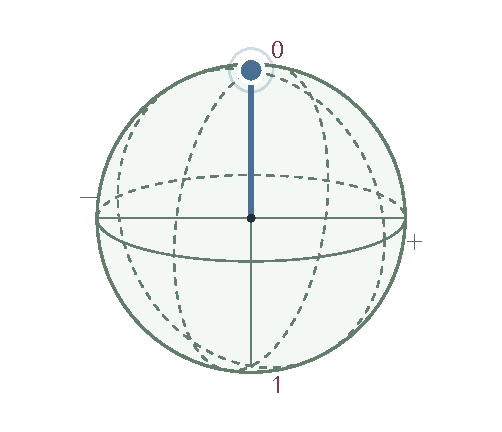
\includegraphics[width=\linewidth,height=94mm,keepaspectratio]{figure/f6e2ab56cb2cc2b36.pdf}\FigureCaption{Preparazione iniziale: sfera modificabile}\end{FigureBlock}
\begin{FigureBlock}\centering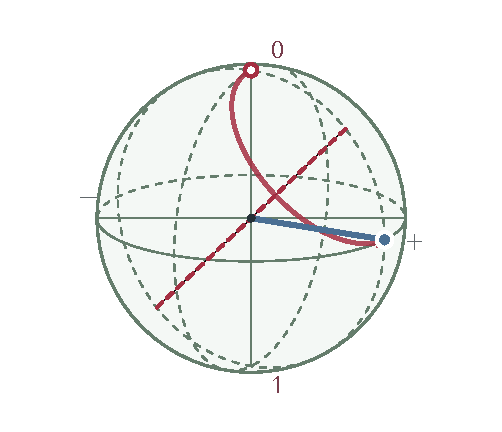
\includegraphics[width=\linewidth,height=94mm,keepaspectratio]{figure/fc2c65a10b1c2d59a.pdf}\FigureCaption{Stato dopo il blocco 1}\end{FigureBlock}
\begin{FigureBlock}\centering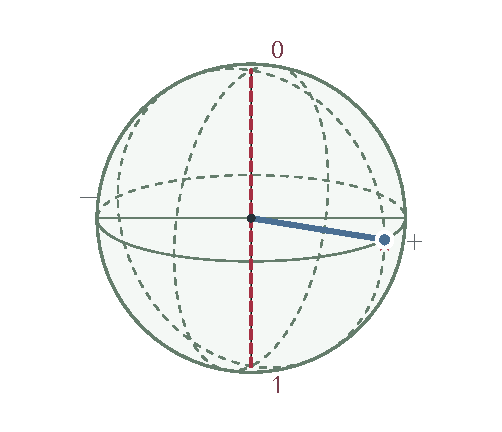
\includegraphics[width=\linewidth,height=94mm,keepaspectratio]{figure/fd04f3209636537e2.pdf}\FigureCaption{Stato dopo il blocco 2}\end{FigureBlock}
\begin{FigureBlock}\centering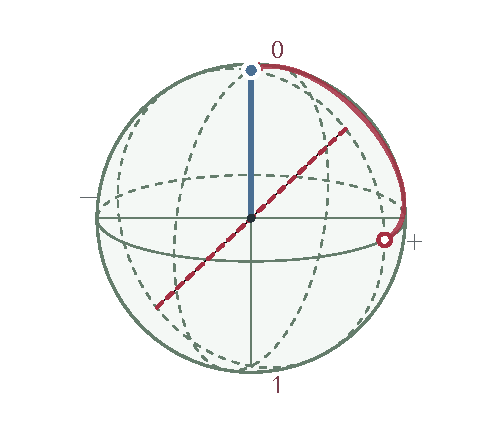
\includegraphics[width=\linewidth,height=94mm,keepaspectratio]{figure/f1e47cb1f015f680d.pdf}\FigureCaption{Stato dopo il blocco 3}\end{FigureBlock}
\begin{FigureBlock}\centering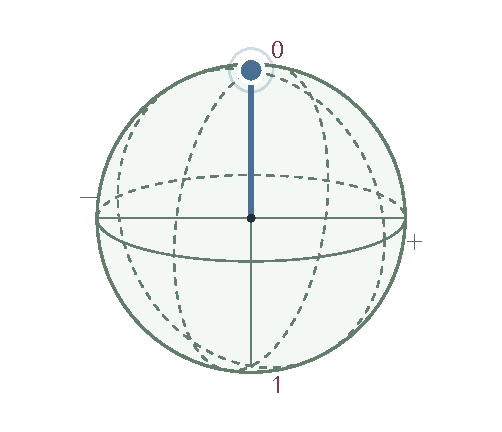
\includegraphics[width=\linewidth,height=94mm,keepaspectratio]{figure/f616a7430b3e5b510.pdf}\FigureCaption{Stato sulla sfera di Bloch}\end{FigureBlock}
\begin{FigureBlock}\centering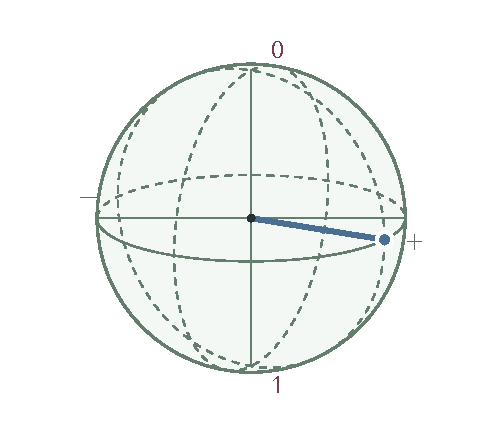
\includegraphics[width=\linewidth,height=94mm,keepaspectratio]{figure/f70a572e97509e0be.pdf}\FigureCaption{Stato sulla sfera di Bloch}\end{FigureBlock}
\begin{FigureBlock}\centering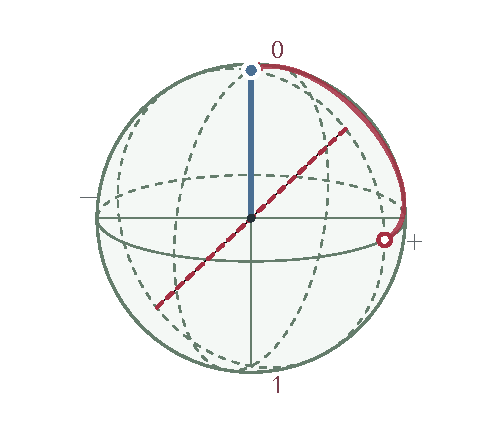
\includegraphics[width=\linewidth,height=94mm,keepaspectratio]{figure/f46cfb2fa0b467aae.pdf}\FigureCaption{Stato sulla sfera di Bloch}\end{FigureBlock}
\begin{FigureBlock}\centering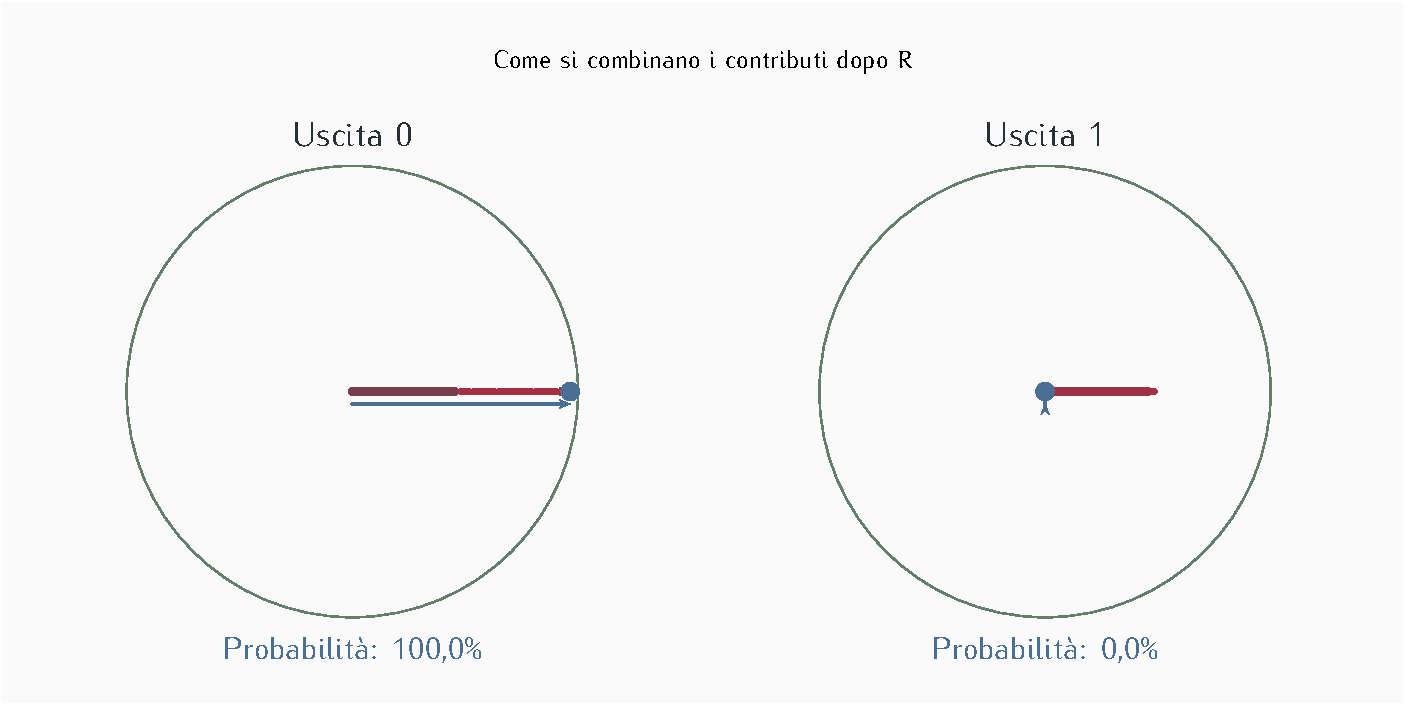
\includegraphics[width=\linewidth,height=94mm,keepaspectratio]{figure/fc2c273ae5cdd6209.pdf}\FigureCaption{Contributi delle componenti \(H\) e \(V\) a ciascuna uscita di \(R\)}\end{FigureBlock}


\BookHeading{\(R\) \(\cdot\) Ricombina le ampiezze}
\(R\) porta 0 nello stato + e 1 nello stato \(- \). Applicata a + dà 0; applicata a \(- \) dà 1. In questo modo rende distinguibili due stati che, misurati direttamente in 0/1, darebbero entrambi 50/50. È la ricombinazione già incontrata nella lezione.\par

In questo passaggio Stato + diventa Stato 0. La curva sulla sfera mostra come agisce l'operazione sullo stato in ingresso.\par

\BookHeading{Prima dell'operazione}
\BookHeading{Dopo \(R\)}
Il cerchio vuoto indica la posizione iniziale; il punto blu indica quella finale. La curva corallo segue la trasformazione sulla sfera. Le percentuali riguardano una misura 0/1 eseguita in quel punto.\par

\BookHeading{Esempi con \(R\)}
La tabella applica soltanto \(R\) a ciascuno stato iniziale. \guillemotleft{}Carica\guillemotright{} prepara quel caso nel primo blocco e lascia I negli altri due, così puoi raccogliere gli esiti e confrontarli con la previsione.\par

\BookHeading{Che cosa significano + e \(- \)}
I due stati occupano punti opposti dell'equatore. Entrambi danno 50/50 nella misura 0/1; la loro fase relativa differisce di mezzo giro. \(R\) porta + in 0 e \(- \) in 1. Questo esempio mostra perché, per prevedere una sequenza di operazioni, occorre conservare anche la fase dello stato.\par

\BookHeading{Come \(R\) ricombina le ampiezze}
Ogni ampiezza in ingresso contribuisce a entrambi gli esiti. Per l'esito 0 i contributi si sommano; per l'esito 1 il secondo contributo cambia verso. Le frecce verde e corallo rappresentano questi contributi, mentre la risultante blu determina la probabilità. Con lo stato + i contributi si rinforzano in 0 e si cancellano in 1; con lo stato \(- \) avviene il contrario.\par

\BookHeading{Eseguire il circuito}
Ogni prova prepara un nuovo qubit nello stato iniziale scelto, applica tutte le operazioni attive e legge 0 oppure 1. Selezionare un passaggio cambia il dettaglio consultato; i conteggi riguardano sempre l'uscita dell'intero circuito.\par

Prove al secondo\par

Regola soltanto la rapidità della raccolta sullo schermo. Le probabilità di ciascuna prova restano le stesse.\par

\BookHeading{Esiti della misura}
La barra colorata mostra la parte della raccolta in cui è comparso ciascun esito: una barra piena corrisponde al 100\%. Il segno verticale indica la probabilità prevista dal modello, anche prima di raccogliere dati.\par

Non sono ancora state eseguite prove. Le barre sono vuote; i segni verticali e le percentuali riportano già ciò che il modello prevede.\par

Ogni prova ripete l'esperimento con una nuova preparazione. Modificare la preparazione o la misura avvia una nuova raccolta: conserva prima il confronto se vuoi ricordare i conteggi precedenti.\par


\BookHeading{Il circuito completo}
Trascina il punto della prima sfera per cambiare la preparazione. Seleziona un blocco per scegliere l'operazione; le caselle modificano direttamente i suoi angoli.\par

Trascina il punto blu.\par

Stato 0\par

Fase\par

Stato +\par

Angolo\par

Stato +\par

Stato 0\par

I conteggi si raccolgono con i pulsanti delle prove.\par

Ogni blocco trasforma lo stato ricevuto da quello precedente. Le sfere mostrano gli stati intermedi calcolati: l'unica misura eseguita è quella finale. La retta corallo indica l'asse della trasformazione; la curva con freccia ne mostra il percorso, dal cerchio vuoto al punto blu. Le fasi dello stato sono riportate fra \(- 180{}^{\circ} \) e \(+180{}^{\circ} \); l'angolo scelto in \(F\) è invece la variazione da applicare. Un segno negativo indica il verso opposto.\par

Ingrandisci la sfera e regola lo stato iniziale\par

\BookHeading{Prepara il punto sulla sfera}
Trascina il punto blu per cambiare la preparazione. Le frecce della tastiera regolano inclinazione e fase; Maiusc riduce il passo, Inizio e Fine selezionano i poli. Al bordo della sfera, ruota la vista per proseguire sull'altro emisfero.\par

0: 100,0\% \(\cdot\) 1: 0,0\% Ai poli è presente una sola componente: la fase relativa non è definita.\par

Muovere il punto cambia lo stato iniziale del qubit. Tutti i blocchi vengono applicati di nuovo a questo stato e la previsione finale si aggiorna insieme alle sfere intermedie. Il tratteggio della freccia indica che il punto si trova sulla metà posteriore della sfera.\par

Distanza angolare dal polo 0\par

Cursore \(\cdot\) Distanza angolare dal polo 0\par

Fase relativa dello stato\par

Cursore \(\cdot\) Fase relativa dello stato\par

Il polo superiore dà 0 con certezza; quello inferiore dà 1 con certezza. Sull'equatore i due esiti hanno la stessa probabilità. Muoversi lungo un parallelo conserva queste probabilità e cambia la fase relativa. Puoi inserire anche una fase negativa: \(- 90{}^{\circ} \) e \(+270{}^{\circ} \) individuano lo stesso punto. Le fasi dello stato sono riportate fra \(- 180{}^{\circ} \) e \(+180{}^{\circ} \); la distanza dal polo 0 varia fra \(0{}^{\circ} \) e \(180{}^{\circ} \).\par


\BookHeading{Che cosa mostra questa configurazione}
Il circuito parte da Stato 0 e arriva a Stato 0. La misura finale prevede 100,00\% di esiti 0 e 0,00\% di esiti 1.\par

Le probabilità si aggiornano quando cambia la preparazione o una delle operazioni. I conteggi si costruiscono avviando le prove; ogni nuova configurazione apre una nuova raccolta.\par

Dopo \(F\), \(R\) ricombina le ampiezze: la fase può così modificare le probabilità finali.\par


Il modello e le sue condizioni\par

Il simulatore descrive uno stato puro mediante due ampiezze, a e b, associate agli esiti 0 e 1. Le probabilità sono i quadrati dei loro moduli. \(X\) scambia a e b; \(Z\) cambia il segno di b; \(Y\) porta la coppia (a, b) in \((- ib\), ia), dove i indica una rotazione di un quarto di giro nel piano delle ampiezze. Una stessa fase applicata a entrambe le ampiezze non modifica lo stato rappresentato sulla sfera.\par

\(R\) calcola \((a+b)/\sqrt{2}\) e \((a- b)/\sqrt{2}\). \(F\) conserva l'ampiezza associata a 0 e ruota quella associata a 1 dell'angolo scelto. La sfera mantiene la rappresentazione geometrica di queste operazioni. I nomi \(X\), \(Y\) e \(Z\) identificano operazioni fissate; il solo angolo regolabile nel circuito è quello di \(F\).\par

Il trascinamento modifica lo stato iniziale e ricalcola tutta la sequenza. Le sfere intermedie sono previsioni del modello; ogni prova genera un esito soltanto alla misura finale, ripartendo ogni volta dalla stessa preparazione. I nomi 0/1 sostituiscono H/V senza modificare il modello matematico.\par


% Authoritative exercise source. Preserve all derivations and diagrams.

\ExerciseStart{G1.10}{Seguire una preparazione sulla sfera di Bloch}{Consolidamento}

\BookHeading{Problema, dati e obiettivo}

Considerare la preparazione \(\ket\psi=(\sqrt3/2)\ket0+(1/2)\ket1\). Ricavarne la rappresentazione di Bloch e studiare l’effetto di una fase \(\pi/2\) sulla seconda componente. Confrontare l’angolo della polarizzazione lineare con quello sulla sfera.

\ExTheory{\ExRef{c1-polarizzazione}{1.05}; \ExRef{c1-calcolo}{1.06}}{Lo stato ha componenti \(\alpha=\cos(\vartheta/2)\) e \(\beta=e^{i\varphi}\sin(\vartheta/2)\). Le coordinate di Bloch sono \(r_x=\sin\vartheta\cos\varphi\), \(r_y=\sin\vartheta\sin\varphi\), \(r_z=\cos\vartheta\). Le probabilità nella base scelta valgono \((1+r_z)/2\) e \((1-r_z)/2\).}

\ExPrediction{La preparazione ha una probabilità maggiore per 0 e si trova nell’emisfero superiore. La variazione della fase descrive una rotazione attorno all’asse verticale, a quota costante.}

\ExFigure{\begin{tikzpicture}[>=Stealth,exlabel,scale=.7]
\draw[Ink!25] (0,0) circle(2);\draw[exaxis] (-2.5,0)--(2.6,0) node[right] {$r_x$};\draw[exaxis] (0,-2.4)--(0,2.6) node[above] {$r_z$};\draw[exvec] (0,0)--(1.73205,1.00000) node[above right] {$ \mathbf r $};\draw[Secondary,->] (0,.7) arc(90:30:.7);\node[right] at (.6,.75) {$\vartheta=60^\circ$};
\end{tikzpicture}}{Sezione meridiana della sfera di Bloch: l’angolo dal polo nord è \(60^\circ\), il doppio dell’angolo lineare della preparazione.}


\begin{ExTasks}

\item Controllare la norma e le probabilità.

\item Ricavare \(\vartheta/2\) dalla prima componente.

\item Calcolare le tre coordinate iniziali.

\item Applicare la fase e ricavare le nuove coordinate.

\item Confrontare angolo di polarizzazione, angolo di Bloch e probabilità finali.

\end{ExTasks}

\ExSolution

\ExStep{Controllare la preparazione}

\ExEq{\|\psi\|^2&=3/4+1/4=1,\quad p_0=3/4,\quad p_1=1/4.}

\ExStep{Ricavare gli angoli}

Poiché \(\cos(\vartheta/2)=\sqrt3/2\) e le due componenti sono positive, \(\vartheta/2=\pi/6\). Dunque \(\vartheta=\pi/3=60^\circ\), mentre \(\varphi=0\). La polarizzazione lineare nel piano H/V forma invece \(30^\circ\).

\ExStep{Costruire il punto sulla sfera}

\ExEq{r_x&=\sin60^\circ\cos0=\sqrt3/2,\\r_y&=\sin60^\circ\sin0=0,\\r_z&=\cos60^\circ=1/2.}
Il controllo \(r_x^2+r_y^2+r_z^2=3/4+0+1/4=1\) colloca il punto sulla superficie unitaria.

\ExStep{Ruotare la fase relativa}

Moltiplicando la seconda componente per \(i\), si ottiene \(\ket{\psi'}=(\sqrt3/2)\ket0+(i/2)\ket1\). Gli angoli diventano \((\vartheta,\varphi)=(\pi/3,\pi/2)\):
\ExEq{\mathbf r'&=(\sin60^\circ\cos90^\circ,\sin60^\circ\sin90^\circ,\cos60^\circ)\\&=(0,\sqrt3/2,1/2).}

\ExStep{Verificare la lettura}

\ExEq{p_0'&=(1+1/2)/2=3/4,\quad p_1'=(1-1/2)/2=1/4.}
Il punto si è spostato sulla sfera, mentre la misura lungo z resta invariata. Un successivo ricombinatore può rendere osservabile la fase cambiata.

\par\noindent\begin{minipage}{\linewidth}
\ExFigure{\begin{tikzpicture}[>=Stealth,exlabel]
\draw[exaxis] (-0.35,0)--(1.55,0) node[right] {$r_x$};\draw[exaxis] (0,-0.35)--(0,1.416025) node[above] {$r_y$};\draw[->,Secondary,line width=1.1pt] (0,0)--(0.866025,0) node[anchor=south west] {$ \varphi=0 $};\draw[->,Accent,line width=1.1pt] (0,0)--(0,0.866025) node[anchor=south west] {$ \varphi=\pi/2 $};\draw[Secondary,dashed] (0,0) circle(.866025);
\end{tikzpicture}}{Proiezione sul piano equatoriale delle coordinate di Bloch; in entrambi i casi \(r_z=1/2\).}


\ExInterpret{La sfera rappresenta stati del qubit e la loro distinguibilità nelle misure. Il raddoppio dell’angolo deriva dalla parametrizzazione con \(\vartheta/2\); non modifica l’orientazione fisica dell’analizzatore.}

\ExLab{Nella sezione 1.05 scegliere orientazione iniziale \(30^\circ\), analizzatore orizzontale e fase V dapprima nulla, poi \(90^\circ\). Osservare la sfera e verificare la probabilità invariata in H/V. Ruotare l’analizzatore per esplorare la sensibilità alla fase.}


\end{minipage}

% Authoritative exercise source. Preserve all derivations and diagrams.

\ExerciseStart{G1.11}{Preparare, introdurre una fase e ricombinare}{Collegamento}

\BookHeading{Problema, dati e obiettivo}

Una preparazione \((1,0)^T\) attraversa un ricombinatore R, uno sfasatore F di \(90^\circ\) e un secondo R. Seguire le due ampiezze e confrontare con fase nulla e mezzo ciclo. R agisce come la porta Hadamard.

\ExTheory{\ExRef{c1-calcolo}{1.06}}{Su una coppia di ampiezze, \(R(\alpha,\beta)^T=((\alpha+\beta)/\sqrt2,(\alpha-\beta)/\sqrt2)^T\). Lo sfasatore applica \(F_\varphi(\alpha,\beta)^T=(\alpha,e^{i\varphi}\beta)^T\). Il modulo quadro di ciascuna componente dà la probabilità.}

\ExPrediction{Il primo R produce due contributi uguali. Con un quarto di ciclo, somma e differenza dei contributi hanno la stessa lunghezza; le due uscite finali dovrebbero essere equiprobabili.}

\ExFigure{\begin{tikzpicture}[>=Stealth,exlabel]
\node[left] at (-.3,0) {$ \ket{0} $};\draw[Ink] (-.3,0)--(4.5,0);\node[draw=Accent,fill=white,minimum height=9mm,minimum width=10mm] at (0.5,0) {$ R $};\node[draw=Accent,fill=white,minimum height=9mm,minimum width=10mm] at (2.0,0) {$ F_{90^\circ} $};\node[draw=Accent,fill=white,minimum height=9mm,minimum width=10mm] at (3.5,0) {$ R $};\node[right] at (4.5,0) {$\ket{\psi_f}$};
\end{tikzpicture}}{Tre trasformazioni consecutive, senza misura fra i blocchi.}


\begin{ExTasks}

\item Applicare il primo R.

\item Moltiplicare la seconda ampiezza per \(i\).

\item Calcolare somma e differenza nell’ultimo R.

\item Calcolare i due moduli quadri.

\item Ripetere per fase 0 e \(\pi\), poi discutere una misura intermedia.

\end{ExTasks}

\ExSolution

\ExStep{Aprire le due componenti}

\ExEq{R\colv{1\\0}&=\colv{(1+0)/\sqrt2\\(1-0)/\sqrt2}=\frac1{\sqrt2}\colv{1\\1}.}

\ExStep{Introdurre un quarto di ciclo}

\ExEq{F_{\pi/2}\frac1{\sqrt2}\colv{1\\1}&=\frac1{\sqrt2}\colv{1\\i}.}
I due moduli quadri sono ancora \(1/2\).

\ExStep{Ricombinare}

\ExEq{R\frac1{\sqrt2}\colv{1\\i}&=\colv{(1/\sqrt2+i/\sqrt2)/\sqrt2\\(1/\sqrt2-i/\sqrt2)/\sqrt2}
=\frac12\colv{1+i\\1-i}.}

\ExStep{Calcolare i conteggi previsti}

\ExEq{p_0&=\frac{(1-i)(1+i)}4=\frac{1+1}4=\frac12,\\p_1&=\frac{(1+i)(1-i)}4=\frac12.}
Su 1000 ripetizioni i conteggi medi sono 500 e 500.

\ExStep{Controllare gli altri due casi}

Con fase nulla, il secondo R riceve \((1,1)^T/\sqrt2\) e produce \((1,0)^T\). Con fase \(\pi\), riceve \((1,-1)^T/\sqrt2\) e produce \((0,1)^T\). Le probabilità passano rispettivamente a \((1,0)\) e \((0,1)\).

\ExStep{Inserire una misura intermedia}

Una misura nella base 0/1 dopo il primo R produce ciascun esito con probabilità \(1/2\). Da \(\ket0\), l’ultimo R dà probabilità \((1/2,1/2)\); da \(\ket1\), anche. Mediando i due rami si ottiene \(p_0=(1/2)(1/2)+(1/2)(1/2)=1/2\), indipendentemente dalla fase. Si tratta di un esperimento differente dal percorso coerente.

\par\noindent\begin{minipage}{\linewidth}
\ExFigure{\begin{tikzpicture}[>=Stealth,exlabel]
\draw[exaxis] (-0.35,0)--(1.55,0) node[right] {$\operatorname{Re}$};\draw[exaxis] (0,-1.35)--(0,1.55) node[above] {$\operatorname{Im}$};\draw[->,Secondary,line width=1.1pt] (0,0)--(1,0) node[anchor=south west] {$ 1 $};\draw[->,Secondary,line width=1.1pt] (0,0)--(0,1) node[anchor=south west] {$ i $};\draw[->,Accent,line width=1.1pt] (0,0)--(1,1) node[anchor=south west] {$ 2\alpha $};\draw[->,Ink,line width=1.1pt] (0,0)--(1,-1) node[anchor=north west] {$ 2\beta $};
\end{tikzpicture}}{Le due diagonali hanno lunghezza \(\sqrt2\); dividendo per due e quadrando si ottiene \(1/2\).}


\ExInterpret{La fase ha un effetto osservabile quando le componenti sono ricombinate. La misura intermedia elimina il termine incrociato nella media dei rami.}

\ExLab{Nella sezione 1.06 caricare R–F–R e impostare la fase a \(90^\circ\). Confrontare poi «Fase nulla», «Mezzo ciclo» e «Misura prima dell’ultima R», seguendo gli stati intermedi senza confondere la loro visualizzazione con una misura.}


\end{minipage}

\Needspace{.43\textheight}
\section{Statistiche locali e correlazioni}
\phantomsection\label{c1-coppie}

{\sffamily\small\color{Ink!70} Riferimento alle slide: p. 246.\par}

{\sffamily\small\color{Ink!70} Laboratorio locale: \nolinkurl{index.html#capitolo-1/coppie}\par}

Una prova produce due risultati, che vanno conservati insieme. Confronteremo preparazioni con gli stessi conteggi individuali e tabelle delle coppie differenti; cambieremo poi la misura per distinguere una scelta casuale da una sovrapposizione.\par


\BookHeading{Preparazione e significato dei comandi}

\BookHeading{Preparare e intervenire}
Sorgente di coppie\par

La sorgente prepara un unico stato congiunto, con contributi uguali delle due alternative indicate. La fase relativa appartiene alla preparazione della coppia.\par

Fase della preparazione congiunta\par

Modifica la relazione di fase fra le due alternative della sovrapposizione. La misura H/V mantiene le stesse coppie possibili; cambiando la misura si può rendere osservabile la fase. Il controllo è inattivo per le miscele e per la preparazione indipendente.\par

Orientazione della misura sul primo\par

\(A_{1}\) è l'uscita lungo la direzione scelta, \(B_{1}\) quella perpendicolare. \(A\) \(0{}^{\circ} \) leggiamo H/V; a \(45{}^{\circ} \) leggiamo \(+45{}^{\circ} /- 45{}^{\circ} \).\par

Orientazione della misura sul secondo\par

\(A_{2}\) e \(B_{2}\) sono le due uscite del secondo analizzatore. Cambiarne l'orientazione cambia la misura sul secondo sistema; la preparazione alla sorgente rimane quella scelta.\par

\BookHeading{La stessa operazione del laboratorio 6}
La lettura sulle diagonali equivale, per queste statistiche, a inserire l'operazione \(R\) su ciascun qubit e misurare poi H/V. Le impostazioni a \(45{}^{\circ} \) riproducono quindi il confronto dopo ricombinazione delle slide.\par


\BookHeading{Figure della configurazione iniziale}
\begin{FigureBlock}\centering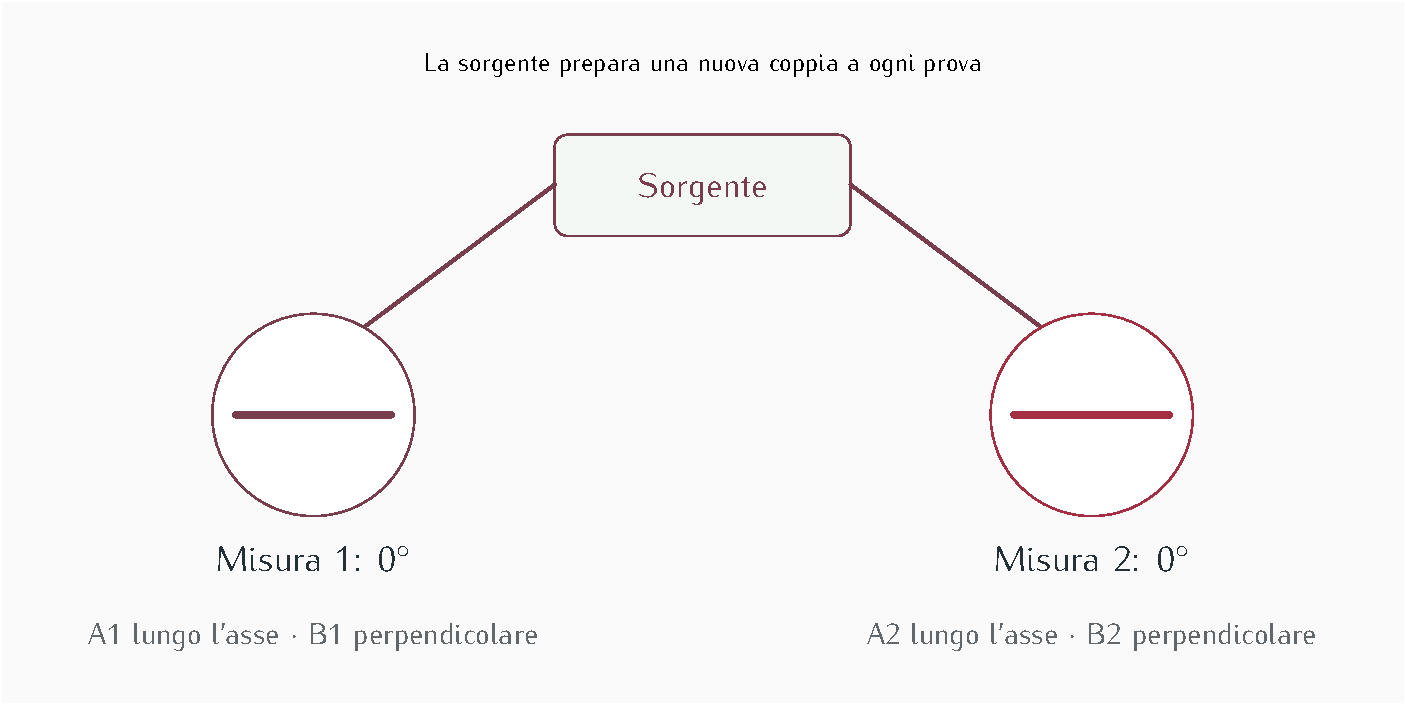
\includegraphics[width=\linewidth,height=94mm,keepaspectratio]{figure/f19fa5b6229d6bfb9.pdf}\FigureCaption{Due analizzatori a 0 e 0 gradi}\end{FigureBlock}

\BookHeading{Esiti della stessa prova \(\cdot\) probabilità prevista e conteggio osservato}
\begingroup\sffamily\fontsize{8.8}{11}\selectfont\setlength{\tabcolsep}{1.6mm}\renewcommand{\arraystretch}{1.28}
\begin{longtable}{>{\RaggedRight\arraybackslash}p{32.421mm}>{\RaggedRight\arraybackslash}p{32.421mm}>{\RaggedRight\arraybackslash}p{32.421mm}>{\RaggedRight\arraybackslash}p{25.937mm}}
\toprule\rowcolor{Accent!7}\BeginAccSupp{method=hex,unicode,ActualText=005000720069006D006F0020002F0020007300650063006F006E0064006F}Primo / secondo\EndAccSupp{} & \BeginAccSupp{method=hex,unicode,ActualText=00412082}\(A_{2}\)\EndAccSupp{} & \BeginAccSupp{method=hex,unicode,ActualText=00422082}\(B_{2}\)\EndAccSupp{} & \BeginAccSupp{method=hex,unicode,ActualText=005000720069006D006F002000730069007300740065006D0061}Primo sistema\EndAccSupp{} \\
\midrule\endfirsthead
\toprule\rowcolor{Accent!7}\BeginAccSupp{method=hex,unicode,ActualText=005000720069006D006F0020002F0020007300650063006F006E0064006F}Primo / secondo\EndAccSupp{} & \BeginAccSupp{method=hex,unicode,ActualText=00412082}\(A_{2}\)\EndAccSupp{} & \BeginAccSupp{method=hex,unicode,ActualText=00422082}\(B_{2}\)\EndAccSupp{} & \BeginAccSupp{method=hex,unicode,ActualText=005000720069006D006F002000730069007300740065006D0061}Primo sistema\EndAccSupp{} \\
\midrule\endhead\bottomrule\endfoot
\BeginAccSupp{method=hex,unicode,ActualText=00412081}\(A_{1}\)\EndAccSupp{} & \BeginAccSupp{method=hex,unicode,ActualText=00350030002C00300025003000200063006F007000700069006500410041}50,0\%0 coppieAA\EndAccSupp{} & \BeginAccSupp{method=hex,unicode,ActualText=0030002C00300025003000200063006F007000700069006500410042}0,0\%0 coppieAB\EndAccSupp{} & \BeginAccSupp{method=hex,unicode,ActualText=00350030002C003000250030002000650073006900740069}50,0\%0 esiti\EndAccSupp{} \\
\BeginAccSupp{method=hex,unicode,ActualText=00422081}\(B_{1}\)\EndAccSupp{} & \BeginAccSupp{method=hex,unicode,ActualText=0030002C00300025003000200063006F007000700069006500420041}0,0\%0 coppieBA\EndAccSupp{} & \BeginAccSupp{method=hex,unicode,ActualText=00350030002C00300025003000200063006F007000700069006500420042}50,0\%0 coppieBB\EndAccSupp{} & \BeginAccSupp{method=hex,unicode,ActualText=00350030002C003000250030002000650073006900740069}50,0\%0 esiti\EndAccSupp{} \\
\BeginAccSupp{method=hex,unicode,ActualText=005300650063006F006E0064006F002000730069007300740065006D0061}Secondo sistema\EndAccSupp{} & \BeginAccSupp{method=hex,unicode,ActualText=00350030002C003000250030002000650073006900740069}50,0\%0 esiti\EndAccSupp{} & \BeginAccSupp{method=hex,unicode,ActualText=00350030002C003000250030002000650073006900740069}50,0\%0 esiti\EndAccSupp{} & \BeginAccSupp{method=hex,unicode,ActualText=00310030003000250030002000700072006F00760065}100\%0 prove\EndAccSupp{} \\
\end{longtable}\endgroup

\BookHeading{Due analizzatori, una registrazione congiunta}
Sovrapposizione HH / VV. La prima lettera di ogni coppia appartiene al primo sistema, la seconda al secondo.\par

Prove al secondo\par

Regola soltanto la rapidità della raccolta sullo schermo. Le probabilità di ciascuna prova restano le stesse.\par

\BookHeading{Leggere una riga del registro}
Esegui una prova per evidenziare la casella corrispondente. Le somme delle righe danno le frequenze del primo sistema; quelle delle colonne danno le frequenze del secondo. I totali individuali non conservano quale esito accompagnasse l'altro.\par

Con \guillemotleft{}Conserva confronto\guillemotright{} puoi mantenere i risultati attuali prima di cambiare sorgente. Per confrontare miscela e sovrapposizione, tieni entrambi gli analizzatori a \(45{}^{\circ} \) e la fase della sovrapposizione a \(0{}^{\circ} \).\par

\BookHeading{Esiti della misura}
La barra colorata mostra la parte della raccolta in cui è comparso ciascun esito: una barra piena corrisponde al 100\%. Il segno verticale indica la probabilità prevista dal modello, anche prima di raccogliere dati.\par

Non sono ancora state eseguite prove. Le barre sono vuote; i segni verticali e le percentuali riportano già ciò che il modello prevede.\par

Ogni prova ripete l'esperimento con una nuova preparazione. Modificare la preparazione o la misura avvia una nuova raccolta: conserva prima il confronto se vuoi ricordare i conteggi precedenti.\par


\BookHeading{Che cosa mostra questa configurazione}
Gli esiti sono concordi nel 100,0\% delle prove e discordi nel 0,0\%. I totali ai margini della tabella mostrano ciò che ciascun osservatore può contare da solo.\par

Con sorgenti concordi e discordi nella lettura H/V, le frequenze individuali sono entrambe 50/50, mentre le coppie occupano caselle diverse. La concordanza in una sola misura può essere prodotta anche da una miscela. Per la sovrapposizione HH/VV con fase nulla, la misura diagonale distingue la preparazione coerente dalla miscela. La possibilità di distinguerle dipende dalla fase e dalla misura.\par

Con fase \(0{}^{\circ} \) e misure \(0{}^{\circ} \) / \(0{}^{\circ} \): la distribuzione coincide con quella della miscela delle stesse alternative. Questo confronto non distingue le preparazioni; la coincidenza riguarda soltanto la misura selezionata.\par


Il modello e le sue condizioni\par

Si calcolano le quattro probabilità della coppia prima di campionare un evento. Le sovrapposizioni hanno due ampiezze di uguale modulo e fase relativa regolabile; le miscele hanno pesi classici uguali. L'interazione guidata è uno scambio condizionato sul secondo qubit. Le orientazioni degli analizzatori definiscono proiezioni su polarizzazioni lineari ortogonali.\par

La preparazione HV/VH è anticorrelata nella base H/V. La sua correlazione in altre basi dipende anche dalla fase: il solo nome \guillemotleft{}anticorrelata\guillemotright{} non implica esiti opposti per qualsiasi misura. Le probabilità locali delle sorgenti congiunte bilanciate restano 50/50. Il confronto dei registri richiede l'associazione degli esiti della stessa prova.\par


% Authoritative exercise source. Preserve all derivations and diagrams.

\ExerciseStart{G1.12}{Ricavare marginali e correlazioni da una tabella congiunta}{Collegamento}

\BookHeading{Problema, dati e obiettivo}

Una sorgente produce esiti binari A e B con probabilità \(P(00)=0{,}4\), \(P(01)=0{,}1\), \(P(10)=0{,}1\), \(P(11)=0{,}4\). Calcolare marginali, probabilità di accordo, correlazione dei valori \(\pm1\) e probabilità condizionata.

\ExTheory{\ExRef{c1-coppie}{1.07}}{La marginale di A si ottiene sommando su B: \(P_A(a)=\sum_bP(a,b)\). Assegnando \(s(0)=+1\), \(s(1)=-1\), la correlazione è \(E=\sum_{a,b}s(a)s(b)P(a,b)\). Per un evento di condizionamento positivo, \(P(B=b\mid A=a)=P(a,b)/P_A(a)\).}

\ExPrediction{Le celle diagonali sono più pesanti. Le due righe e le due colonne hanno la stessa somma: ciascun osservatore isolato vedrà esiti uniformi.}

\ExFigure{\begin{tikzpicture}[>=Stealth,exlabel]
\foreach \x/\y/\v in {0/1/.4,1.5/1/.1,0/0/.1,1.5/0/.4}{\node[draw=Secondary,minimum width=15mm,minimum height=10mm] at (\x,\y) {$\v$};}\node at (0,1.9) {$B=0$};\node at (1.5,1.9) {$B=1$};\node[left] at (-1,1) {$A=0$};\node[left] at (-1,0) {$A=1$};
\end{tikzpicture}}{Tabella congiunta. Le righe raggruppano gli esiti di A, le colonne quelli di B.}


\begin{ExTasks}

\item Controllare che la somma delle quattro celle sia uno.

\item Sommare righe e colonne.

\item Calcolare accordo e disaccordo.

\item Attribuire i segni ai quattro termini di E.

\item Calcolare \(P(B=0\mid A=0)\) e confrontare con una sorgente indipendente.

\end{ExTasks}

\ExSolution

\ExStep{Normalizzare la tabella}

\ExEq{0{,}4+0{,}1+0{,}1+0{,}4=1.}
Tutte le celle sono non negative; la tabella definisce una distribuzione congiunta.

\ExStep{Ricavare le marginali}

\ExEq{P_A(0)&=0{,}4+0{,}1=0{,}5,\quad P_A(1)=0{,}1+0{,}4=0{,}5,\\P_B(0)&=0{,}4+0{,}1=0{,}5,\quad P_B(1)=0{,}1+0{,}4=0{,}5.}

\ExStep{Confrontare coppie uguali e diverse}

\ExEq{P(A=B)&=P(00)+P(11)=0{,}8,\\P(A\ne B)&=P(01)+P(10)=0{,}2.}
Su 500 coppie si attendono in media 400 accordi e 100 disaccordi.

\ExStep{Calcolare la correlazione}

I prodotti dei segni sono \(+1,-1,-1,+1\). Pertanto
\ExEq{E&=0{,}4-0{,}1-0{,}1+0{,}4=0{,}6\\&=P(A=B)-P(A\ne B)=0{,}8-0{,}2.}

\ExStep{Condizionare e confrontare}

\ExEq{P(B=0\mid A=0)&=\frac{0{,}4}{0{,}5}=0{,}8.}
Per due esiti indipendenti con le stesse marginali, ciascuna cella varrebbe \(0{,}5\cdot0{,}5=0{,}25\), la probabilità di accordo sarebbe \(1/2\) ed E sarebbe zero. Le marginali coincidono nei due modelli, le correlazioni differiscono.

\par\noindent\begin{minipage}{\linewidth}
\ExFigure{\begin{tikzpicture}[>=Stealth,exlabel]
\draw[exaxis] (-.6,0)--(4.4,0) node[right] {esito};\draw[exaxis] (-.6,0)--(-.6,3.6) node[above] {$p$};\node[left] at (-.6,3) {$ 1 $};\draw[Ink!15,dashed] (-.6,3)--(3.9000000000000004,3);\filldraw[fill=Accent!25,draw=Accent] (0.0,0) rectangle (0.65,1.2000000000000002);\node[below] at (0.325,0) {$ 00 $};\node[above] at (0.325,1.2000000000000002) {$ 0.4 $};\filldraw[fill=Accent!25,draw=Accent] (1.1,0) rectangle (1.75,0.30000000000000004);\node[below] at (1.425,0) {$ 01 $};\node[above] at (1.425,0.30000000000000004) {$ 0.1 $};\filldraw[fill=Accent!25,draw=Accent] (2.2,0) rectangle (2.85,0.30000000000000004);\node[below] at (2.5250000000000004,0) {$ 10 $};\node[above] at (2.5250000000000004,0.30000000000000004) {$ 0.1 $};\filldraw[fill=Accent!25,draw=Accent] (3.3000000000000003,0) rectangle (3.95,1.2000000000000002);\node[below] at (3.6250000000000004,0) {$ 11 $};\node[above] at (3.6250000000000004,1.2000000000000002) {$ 0.4 $};
\end{tikzpicture}}{Le quattro probabilità prima di qualunque raggruppamento.}


\ExInterpret{Una tabella in una sola base può essere riprodotta da una sorgente classica correlata. L’entanglement richiede informazioni ulteriori sulla preparazione e sulle misure in altre basi.}

\ExLab{Nella sezione 1.07 confrontare «Indipendenti», «Concordi in H/V» e «Discordi in H/V», calcolando marginali ed E dalle rispettive tabelle. La distribuzione dell’esercizio è una miscela con peso \(0{,}6\) della sorgente concorde e peso \(0{,}4\) di quella indipendente: le celle diagonali sono \(0{,}6/2+0{,}4/4=0{,}4\), le altre \(0{,}4/4=0{,}1\).}


\end{minipage}

\Needspace{.43\textheight}
\section{Una coppia entangled incontra l'ambiente}
\phantomsection\label{c1-ambiente}

{\sffamily\small\color{Ink!70} Riferimento alle slide: p. 277.\par}

{\sffamily\small\color{Ink!70} Laboratorio locale: \nolinkurl{index.html#capitolo-1/ambiente}\par}

Riprendiamo la coppia entangled del laboratorio precedente, preparata in modo che \(H\) e \(V\) compaiano con uguale probabilità e che i due esiti siano concordi. Facciamo interagire il secondo sistema con l'ambiente e osserviamo soltanto la coppia. L'ambiente può conservare una traccia diversa a seconda della componente \(H\) o \(V\) con cui ha interagito: al crescere di questa distinzione, la coppia perde la coerenza iniziale.\par


\BookHeading{Preparazione e significato dei comandi}

\BookHeading{Preparare e intervenire}
Accoppiamento con l'ambiente\par

Questo comando regola quanto le due alternative \(H\) e \(V\) del secondo sistema lasciano tracce differenti nell'ambiente. \(A\) 0 la coppia è isolata. \(A\) 100 le tracce sono completamente distinguibili; i valori intermedi descrivono un'interazione parziale. La scala da 0 a 100 è una regolazione del modello: al valore 50 l'indicatore di coerenza residua vale circa 71\%. Il comando regola l'interazione, mentre l'indicatore sottostante ne quantifica l'effetto. Tutte le coppie arrivano ai rivelatori.\par

\BookHeading{Scegliere che cosa misurare}
I due analizzatori vengono orientati nello stesso modo. La scelta cambia la domanda posta alla coppia dopo l'interazione.\par

H/V distingue orizzontale e verticale. La lettura diagonale distingue le polarizzazioni \(+45{}^{\circ} \) e \(- 45{}^{\circ} \), indicate nei conteggi con + e \(- \). Il primo simbolo di ciascun esito riguarda il sistema 1, il secondo il sistema 2.\par

\BookHeading{Una sequenza da provare}
Il confronto iniziale usa 10.000 prove diagonali sulla coppia isolata. Ripetendo la raccolta con accoppiamento 100 compaiono anche esiti discordi. La lettura H/V, alle stesse condizioni di accoppiamento, conserva invece la concordanza: la differenza fra le due misure permette di riconoscere quale informazione sia divenuta inaccessibile nella descrizione della sola coppia.\par


\BookHeading{Figure della configurazione iniziale}
\begin{FigureBlock}\centering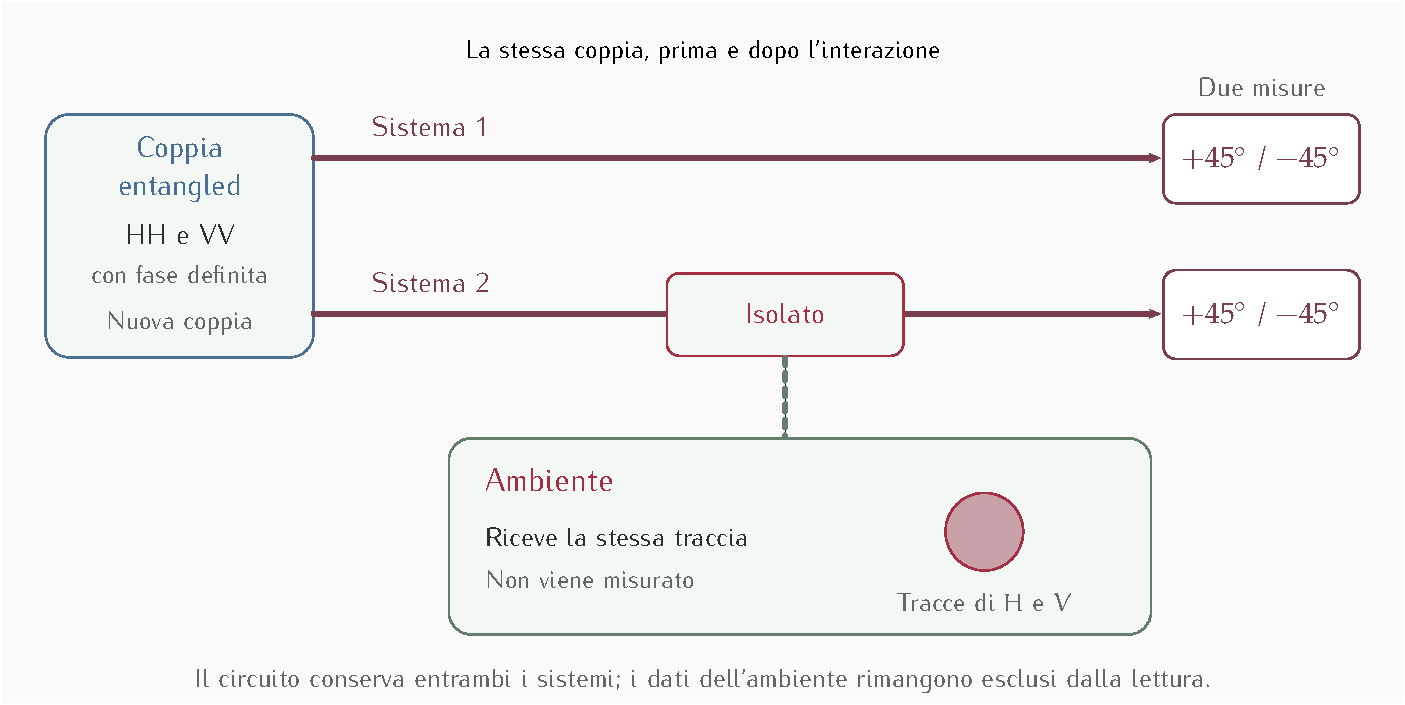
\includegraphics[width=\linewidth,height=94mm,keepaspectratio]{figure/f9c1abf2280a9eb3c.pdf}\FigureCaption{Coppia entangled: il secondo sistema interagisce con l'ambiente; intensità 0 su 100. Entrambi sono poi misurati lungo le diagonali}\end{FigureBlock}


Le due linee seguono i membri della coppia. Soltanto il secondo incontra l'ambiente, rappresentato dal riquadro corallo. I cerchi indicano in modo qualitativo quanto le due tracce siano distinguibili; la loro area di sovrapposizione non è una scala di probabilità.\par

\BookHeading{Dove si vede la perdita di coerenza}
La misura H/V continua a produrre soltanto HH e VV, anche quando l'ambiente li distingue completamente. La misura diagonale è sensibile alla relazione di fase fra queste alternative: per la coppia isolata i due esiti sono sempre concordi; aumentando l'interazione compaiono \(+- \) e \(- +\), fino a rendere i quattro esiti equiprobabili.\par

\BookHeading{La correlazione rimane}
Esiti concordi HH oppure VV\par

\BookHeading{La coerenza diventa osservabile}
Esiti concordi ++ oppure \(- - \)\par

È un indicatore del modello, riferito alla relazione fra HH e VV. Al 100\% la fase iniziale è interamente disponibile nelle misure della coppia; allo 0\% la coppia ha perso questa coerenza. Nella lettura diagonale, l'indicatore è la differenza fra la percentuale di esiti concordi e quella di esiti discordi.\par

\BookHeading{Dalle previsioni ai conteggi}
Ogni prova registra entrambi i risultati della stessa coppia. Per esempio, \(+- \) significa \(+45{}^{\circ} \) sul primo sistema e \(- 45{}^{\circ} \) sul secondo. Aumentando il numero di prove, le frequenze tendono ai valori riportati nella colonna \guillemotleft{}Dopo l'interazione\guillemotright{}.\par

Considerato singolarmente, ciascun sistema continua a dare due esiti equiprobabili in entrambe le letture. Per osservare la variazione occorre conservare l'associazione fra i due risultati e confrontare le coppie.\par

Prove al secondo\par

Regola soltanto la rapidità della raccolta sullo schermo. Le probabilità di ciascuna prova restano le stesse.\par

\BookHeading{Conteggi dopo l'interazione}
La barra colorata mostra la parte della raccolta in cui è comparso ciascun esito: una barra piena corrisponde al 100\%. Il segno verticale indica la probabilità prevista dal modello, anche prima di raccogliere dati.\par

Non sono ancora state eseguite prove. Le barre sono vuote; i segni verticali e le percentuali riportano già ciò che il modello prevede.\par

Ogni prova ripete l'esperimento con una nuova preparazione. Modificare la preparazione o la misura avvia una nuova raccolta: conserva prima il confronto se vuoi ricordare i conteggi precedenti.\par


\BookHeading{Che cosa mostra questa configurazione}
Con l'interazione a 0 su 100, la misura diagonale dà esiti concordi nel 100,0\% delle prove e discordi nel 0,0\%. Il valore si riferisce alle probabilità; una raccolta finita può discostarsene.\par

La coppia isolata conserva la fase della preparazione e mostra concordanza perfetta sia in H/V sia sulle diagonali.\par

Questa riduzione della coerenza nella descrizione della coppia è la decoerenza. Il modello conserva la descrizione quantistica dell'insieme formato dalla coppia e dall'ambiente; osservare soltanto i due sistemi lascia fuori le correlazioni sviluppate con l'ambiente.\par


Il modello e le sue condizioni\par

La preparazione iniziale è la sovrapposizione coerente ed equiprobabile di HH e VV, con fase relativa nulla. Il secondo qubit interagisce con un ambiente inizialmente puro: \(H\) lascia l'ambiente invariato, \(V\) ne ruota lo stato di un angolo proporzionale al comando, da \(0{}^{\circ} \) a \(90{}^{\circ} \). Quando le due tracce diventano distinguibili, le probabilità della sola coppia si avvicinano a quelle di una scelta casuale fra HH e VV. Il programma calcola le probabilità della coppia sommando su tutti gli esiti dell'ambiente, che qui non viene letto.\par

Il modello descrive una perdita di coerenza rispetto alle componenti HH e VV senza assorbimento né rilassamento. L'indicatore riportato vale 1 per tracce identiche e 0 per tracce ortogonali; coincide con il contrasto fra esiti concordi e discordi nella lettura diagonale. L'interazione rappresenta una possibile causa di decoerenza: altre interazioni possono produrre comportamenti differenti.\par

Ogni prova usa una nuova coppia e un ambiente preparato nello stesso stato iniziale. Ridurre il comando cambia l'interazione delle prove successive; non ricostruisce lo stato delle coppie già misurate. Con tracce completamente distinguibili, la coppia è una miscela separabile di HH e VV. Le letture mostrate si riferiscono a questa famiglia di stati e non costituiscono una verifica universale dell'entanglement.\par


% Authoritative exercise source. Preserve all derivations and diagrams.

\ExerciseStart{G1.13}{Seguire l'effetto di un'interazione con l'ambiente}{Collegamento}

\BookHeading{Problema, dati e obiettivo}

Una coppia inizialmente concorde e coerente interagisce con un ambiente. Lo stato complessivo è \((\ket{00}\ket{e_0}+\ket{11}\ket{e_1})/\sqrt2\), dove le due tracce ambientali sono normalizzate e hanno sovrapposizione reale \(\gamma=\langle e_0|e_1\rangle\). Calcolare le probabilità nelle basi Z,Z e X,X per \(\gamma=1,1/2,0\).

\ExTheory{\ExRef{c1-ambiente}{1.08}}{La base X è \(\ket\pm=(\ket0\pm\ket1)/\sqrt2\). Il quadrato della lunghezza della somma di due vettori ambientali unitari è \(\|e_0+e_1\|^2=2+2\gamma\); quello della differenza è \(2-2\gamma\). La sovrapposizione \(\gamma\) misura quanto le tracce siano distinguibili.}

\ExPrediction{Se le tracce coincidono, i contributi possono interferire completamente. Se sono ortogonali, la norma della loro somma non contiene un termine incrociato. Prevedere quali correlazioni siano sensibili a questo cambiamento.}

\ExFigure{\begin{tikzpicture}[>=Stealth,exlabel]
\draw[exaxis] (-0.35,0)--(1.55,0) node[right] {$x_1$};\draw[exaxis] (0,-0.35)--(0,1.416025) node[above] {$x_2$};\draw[->,Secondary,line width=1.1pt] (0,0)--(1,0) node[anchor=south west] {$ e_0 $};\draw[->,Accent,line width=1.1pt] (0,0)--(0.5,0.866025) node[anchor=south west] {$ e_1 $};
\end{tikzpicture}}{Piano reale che rappresenta due tracce ambientali con \(\gamma=\cos60^\circ=1/2\). La proiezione distingue sovrapposizione e ortogonalità.}


\begin{ExTasks}

\item Calcolare le probabilità dei due rami in Z,Z.

\item Espandere \(\ket{00}\) e \(\ket{11}\) nella base X,X.

\item Raccogliere i vettori ambientali per ciascun esito.

\item Calcolare le quattro probabilità in funzione di \(\gamma\).

\item Valutare i tre casi e controllare le marginali.

\end{ExTasks}

\ExSolution

\ExStep{Leggere nella base Z}

I rami \(00\) e \(11\) hanno ampiezza di norma \(1/\sqrt2\). Pertanto \(P(00)=P(11)=1/2\) e \(P(01)=P(10)=0\), qualunque sia \(\gamma\).

\ExStep{Cambiare base}

Dalle inverse \(\ket0=(\ket+ +\ket-)/\sqrt2\) e \(\ket1=(\ket+ -\ket-)/\sqrt2\),
\ExEq{\ket{00}&=\tfrac12(\ket{++}+\ket{+-}+\ket{-+}+\ket{--}),\\\ket{11}&=\tfrac12(\ket{++}-\ket{+-}-\ket{-+}+\ket{--}).}

\ExStep{Raccogliere le ampiezze ambientali}

Sostituendo nello stato complessivo, gli esiti \(++\) e \(--\) hanno vettore ambientale \((e_0+e_1)/(2\sqrt2)\); gli esiti \(+-\) e \(-+\) hanno \((e_0-e_1)/(2\sqrt2)\).

\ExStep{Calcolare i moduli quadri}

\ExEq{\|e_0\pm e_1\|^2&=\langle e_0|e_0\rangle+\langle e_1|e_1\rangle
\pm\langle e_0|e_1\rangle\pm\langle e_1|e_0\rangle\\&=1+1\pm\gamma\pm\gamma=2\pm2\gamma,\\P(++)=P(--)&=(2+2\gamma)/8=(1+\gamma)/4,\\P(+-)=P(-+)&=(1-\gamma)/4.}

\ExStep{Valutare e controllare}

Per \(\gamma=1\) le probabilità sono \((1/2,0,0,1/2)\). Per \(\gamma=1/2\) sono \((3/8,1/8,1/8,3/8)\). Per \(\gamma=0\) sono tutte \(1/4\). In ogni caso una riga somma \((1+\gamma)/4+(1-\gamma)/4=1/2\); entrambe le marginali restano uniformi. La correlazione X,X è \(2(1+\gamma)/4-2(1-\gamma)/4=\gamma\).

\par\noindent\begin{minipage}{\linewidth}
\ExFigure{\begin{tikzpicture}[>=Stealth,exlabel]
\draw[exaxis] (-.6,0)--(4.4,0) node[right] {esito};\draw[exaxis] (-.6,0)--(-.6,3.6) node[above] {$p$};\node[left] at (-.6,3) {$ 1 $};\draw[Ink!15,dashed] (-.6,3)--(3.9000000000000004,3);\filldraw[fill=Accent!25,draw=Accent] (0.0,0) rectangle (0.65,1.125);\node[below] at (0.325,0) {$ ++ $};\node[above] at (0.325,1.125) {$ 0.375 $};\filldraw[fill=Accent!25,draw=Accent] (1.1,0) rectangle (1.75,0.375);\node[below] at (1.425,0) {$ +- $};\node[above] at (1.425,0.375) {$ 0.125 $};\filldraw[fill=Accent!25,draw=Accent] (2.2,0) rectangle (2.85,0.375);\node[below] at (2.5250000000000004,0) {$ -+ $};\node[above] at (2.5250000000000004,0.375) {$ 0.125 $};\filldraw[fill=Accent!25,draw=Accent] (3.3000000000000003,0) rectangle (3.95,1.125);\node[below] at (3.6250000000000004,0) {$ -- $};\node[above] at (3.6250000000000004,1.125) {$ 0.375 $};
\end{tikzpicture}}{Probabilità in X,X per sovrapposizione ambientale \(1/2\).}


\ExInterpret{L’informazione trasferita all’ambiente modifica le correlazioni accessibili sulla coppia. La descrizione complessiva conserva le ampiezze; ignorare l’ambiente richiede sommare correttamente i suoi contributi ortogonali.}

\ExLab{Nella sezione 1.08 confrontare «Coppia isolata», «Interazione parziale» e «Tracce distinguibili». Leggere il valore della sovrapposizione ambientale e sostituirlo nelle formule ottenute. Passare da H/V a \(+45^\circ/-45^\circ\), confrontando marginali e correlazioni.}


\end{minipage}

\Needspace{.43\textheight}
\section{Quali dati servono per continuare?}
\phantomsection\label{c1-informazione}

{\sffamily\small\color{Ink!70} Riferimento alle slide: p. 300.\par}

{\sffamily\small\color{Ink!70} Laboratorio locale: \nolinkurl{index.html#capitolo-1/informazione}\par}

Per continuare il calcolo dopo un'interruzione occorre registrare informazioni sufficienti sulle operazioni ancora da eseguire. Confronteremo un archivio che conserva il punto sulla sfera con uno che conserva soltanto le probabilità 0/1. La geometria mostrerà quali preparazioni diventano indistinguibili nel secondo archivio.\par


\BookHeading{Preparazione e significato dei comandi}

\BookHeading{Preparare e intervenire}
Contenuto del prossimo archivio\par

Il primo archivio conserva la probabilità di 0; quella di 1 si ottiene per differenza dal totale. Il secondo conserva le tre coordinate del punto, che includono anche la fase. Sono dati già noti al programma che ha preparato la simulazione.\par

Il riferimento originale resta separato, per verificare le previsioni dopo la ricarica. La ricostruzione non vi accede. \guillemotleft{}Prepara un nuovo stato\guillemotright{} riapre una sessione di lavoro lasciando disponibile l'archivio esistente.\par

Operazione dopo la ricarica\par

\(R\) porta 0 nello stato + e 1 nello stato \(- \). Applicata a + dà 0; applicata a \(- \) dà 1. In questo modo rende distinguibili due stati che, misurati direttamente in 0/1, darebbero entrambi 50/50. È la ricombinazione già incontrata nella lezione.\par


\BookHeading{Figure della configurazione iniziale}
\begin{FigureBlock}\centering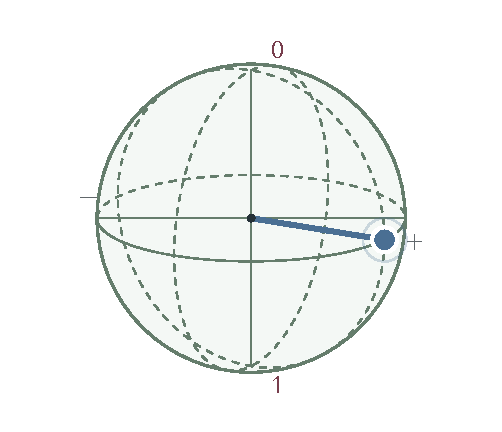
\includegraphics[width=\linewidth,height=94mm,keepaspectratio]{figure/fe4af1e191385e86b.pdf}\FigureCaption{Stato sulla sfera di Bloch}\end{FigureBlock}


\BookHeading{Lo stato che il programma sta usando}
Il punto iniziale prepara Stato +: 0 con probabilità 50,0\%, 1 con probabilità 50,0\%. Muovi il punto per scegliere anche probabilità intermedie.\par

\BookHeading{Prepara il punto sulla sfera}
Trascina il punto blu per cambiare la preparazione. Le frecce della tastiera regolano inclinazione e fase; Maiusc riduce il passo, Inizio e Fine selezionano i poli. Al bordo della sfera, ruota la vista per proseguire sull'altro emisfero.\par

0: 50,0\% \(\cdot\) 1: 50,0\% Fase relativa \(0{,}0{}^{\circ} \)\par

Muovere il punto cambia lo stato iniziale del qubit. Tutti i blocchi vengono applicati di nuovo a questo stato e la previsione finale si aggiorna insieme alle sfere intermedie. Il tratteggio della freccia indica che il punto si trova sulla metà posteriore della sfera.\par

Distanza angolare dal polo 0\par

Cursore \(\cdot\) Distanza angolare dal polo 0\par

Fase relativa dello stato\par

Cursore \(\cdot\) Fase relativa dello stato\par

Il polo superiore dà 0 con certezza; quello inferiore dà 1 con certezza. Sull'equatore i due esiti hanno la stessa probabilità. Muoversi lungo un parallelo conserva queste probabilità e cambia la fase relativa. Puoi inserire anche una fase negativa: \(- 90{}^{\circ} \) e \(+270{}^{\circ} \) individuano lo stesso punto. Le fasi dello stato sono riportate fra \(- 180{}^{\circ} \) e \(+180{}^{\circ} \); la distanza dal polo 0 varia fra \(0{}^{\circ} \) e \(180{}^{\circ} \).\par

\BookHeading{Il contenuto effettivo del file}
Importa un archivio\par

La chiave pH indica la probabilità di \(H\), cioè 0; vector contiene le coordinate del punto. Il contenuto visualizzato coincide con il file esportato. I risultati delle prove hanno un'esportazione separata.\par


\BookHeading{Che cosa mostra questa configurazione}
La sequenza di registrazione, chiusura e ricarica permette di verificare se i dati conservati bastano per prevedere l'operazione scelta.\par


Il modello e le sue condizioni\par

Si salva uno stato puro noto al simulatore classico. L'archivio ridotto contiene la probabilità teorica esatta di 0, così da separare la perdita della fase dall'imprecisione statistica di una stima. Le ricostruzioni sono i punti della sfera con quella stessa probabilità; gli estremi delle previsioni sono calcolati sull'intero parallelo.\par

Il file ridotto non include fase o nome della preparazione. Il riferimento usato per il controllo resta esterno alla procedura di ricostruzione. Su un qubit fisico sconosciuto, una singola misura non rende disponibile l'intero stato. La registrazione qui esaminata riguarda dati già presenti nel programma.\par


% Authoritative exercise source. Preserve all derivations and diagrams.

\ExerciseStart{G1.14}{Stabilire quali dati servano alla previsione successiva}{Collegamento}

\BookHeading{Problema, dati e obiettivo}

Due archivi registrano soltanto le probabilità \((1/2,1/2)\) nella base 0/1. Le preparazioni originali erano \(\ket+=(\ket0+\ket1)/\sqrt2\) e \(\ket-=(\ket0-\ket1)/\sqrt2\). Stabilire se gli archivi consentano di prevedere una successiva Hadamard.

\ExTheory{\ExRef{c1-informazione}{1.09}}{La regola di Born conserva il modulo di ogni ampiezza e perde la sua fase. La trasformazione H forma somma e differenza: \(H(\alpha,\beta)^T=((\alpha+\beta)/\sqrt2,(\alpha-\beta)/\sqrt2)^T\). Una fase globale comune non cambia una previsione di misura.}

\ExPrediction{I vettori reali delle due preparazioni sono ortogonali, benché i quadrati delle componenti coincidano. La ricombinazione può separare le loro previsioni.}

\ExFigure{\begin{tikzpicture}[>=Stealth,exlabel]
\draw[exaxis] (-0.35,0)--(1.55,0) node[right] {$x_1$};\draw[exaxis] (0,-1.0571)--(0,1.2570999999999999) node[above] {$x_2$};\draw[->,Accent,line width=1.1pt] (0,0)--(0.7071,0.7071) node[anchor=south west] {$ + $};\draw[->,Secondary,line width=1.1pt] (0,0)--(0.7071,-0.7071) node[anchor=north west] {$ - $};
\end{tikzpicture}}{Piano reale delle ampiezze: i due vettori hanno componenti di uguale modulo e sono ortogonali.}


\begin{ExTasks}

\item Calcolare le probabilità dei due stati iniziali.

\item Applicare H a \(\ket+\).

\item Applicare H a \(\ket-\).

\item Confrontare con una miscela equiprobabile delle due preparazioni.

\item Indicare quali dati aggiuntivi rendano possibile la previsione.

\end{ExTasks}

\ExSolution

\ExStep{Confrontare gli archivi}

Per \(\ket+\), i quadrati sono \((1/\sqrt2)^2=1/2\) e \((1/\sqrt2)^2=1/2\). Per \(\ket-\), il secondo è \((-1/\sqrt2)^2=1/2\). I dati registrati coincidono.

\ExStep{Trasformare la preparazione positiva}

\ExEq{H\ket+&=\frac12\colv{1+1\\1-1}=\colv{1\\0}=\ket0.}
La probabilità finale di zero è uno.

\ExStep{Trasformare la preparazione negativa}

\ExEq{H\ket-&=\frac12\colv{1-1\\1+1}=\colv{0\\1}=\ket1.}
La probabilità finale di zero è nulla.

\ExStep{Esaminare una ricostruzione possibile}

Se si assumesse una miscela che sceglie \(\ket+\) e \(\ket-\) con uguale probabilità, la media dopo H sarebbe
\ExEq{P(0)&=\tfrac12\cdot1+\tfrac12\cdot0=\tfrac12,\\P(1)&=\tfrac12\cdot0+\tfrac12\cdot1=\tfrac12.}
Questa è una terza preparazione compatibile con i dati iniziali dell’archivio.

\ExStep{Identificare l’informazione necessaria}

Per uno stato puro normalizzato basterebbero le due probabilità e la fase relativa, che vale 0 nel primo caso e \(\pi\) nel secondo. Moltiplicare entrambe le componenti per lo stesso \(e^{i\chi}\) moltiplica anche lo stato finale per quel fattore e lascia invariati i moduli quadri.

\par\noindent\begin{minipage}{\linewidth}
\ExFigure{\begin{tikzpicture}[>=Stealth,exlabel]
\node[exbox] (n0) at (0.0,0.0) {$\ket+\xrightarrow{H}\ket0$};\node[exbox] (n1) at (3.6,0.0) {$P(0)=1$};\draw[exother] (n0)--(n1);\node[exbox] (n2) at (7.2,0.0) {fase relativa $0$};\draw[exother] (n1)--(n2);\node[exbox] (n3) at (0.0,-1.6) {$\ket-\xrightarrow{H}\ket1$};\draw[exother] (n2.south)--++(0,-.4)-|(n3.north);\node[exbox] (n4) at (3.6,-1.6) {$P(0)=0$};\draw[exother] (n3)--(n4);\node[exbox] (n5) at (7.2,-1.6) {fase relativa $\pi$};\draw[exother] (n4)--(n5);
\end{tikzpicture}}{Due previsioni incompatibili a partire dalle medesime probabilità iniziali.}


\ExInterpret{L’archivio delle probabilità di una sola misura non determina in generale lo stato. Le fasi relative consentono di calcolare le interferenze successive; per preparazioni miste occorre una descrizione statistica più generale.}

\ExLab{Nella sezione 1.09 confrontare «Diagonale · sole probabilità» e «Diagonale · stato completo». Registrare, chiudere e ricaricare lo stato, quindi applicare il ricombinatore. Confrontare la previsione ricaricata con quella della preparazione originale e leggere quale ricostruzione adotti l’archivio incompleto.}


\end{minipage}

\Needspace{.43\textheight}
\section{Stessi conteggi, cause differenti}
\phantomsection\label{c1-sintesi}

{\sffamily\small\color{Ink!70} Riferimento alle slide: p. 308.\par}

{\sffamily\small\color{Ink!70} Laboratorio locale: \nolinkurl{index.html#capitolo-1/sintesi}\par}

Due apparati producono inizialmente gli stessi conteggi \(D_{1}/D_{2}\) per qualunque fase impostata. Vogliamo verificare se questa osservazione basti a descriverne il funzionamento. Sono disponibili due interventi: stabilizzare la fase fra le prove e compensare un'eventuale traccia dei cammini nell'ambiente. Confrontandone gli effetti potremo distinguere le spiegazioni considerate nel modello.\par


\BookHeading{Preparazione e significato dei comandi}

\BookHeading{Preparare e intervenire}
Fase nominale dell'interferometro\par

È la differenza di fase impostata fra i due cammini. La scansione ripete la raccolta a tredici valori, da \(0{}^{\circ} \) a \(360{}^{\circ} \), per verificare come cambia la probabilità di \(D_{1}\).\par

Stabilizza la fase fra le prove\par

Rende ripetibile la fase impostata, eliminando le sue eventuali variazioni casuali da una preparazione alla successiva. Agisce sul ritardo relativo; una traccia già presente nell'ambiente resta disponibile.\par

Compensa la traccia dei cammini\par

Applica l'inversa dell'interazione di marcatura presente nell'apparato, prima dell'ultima \(R\). Se i cammini avevano lasciato tracce diverse, questa operazione le riporta allo stesso stato. Le eventuali variazioni casuali della fase rimangono.\par

Mostra anche la polarizzazione dell'ambiente\par

Suddivide gli stessi eventi secondo la lettura H/V della traccia: \(D_{1}\cdot H\), \(D_{1}\cdot V\), \(D_{2}\cdot H\), \(D_{2}\cdot V\). Il comando cambia il raggruppamento del registro; i totali \(D_{1}/D_{2}\) restano gli stessi. Qui la polarizzazione realizza l'ambiente controllabile incontrato nel laboratorio 08.\par

Registra impostazioni e conteggi delle prove a fase fissata. La scansione completa si esporta dal proprio grafico.\par


\BookHeading{Figure della configurazione iniziale}
\begin{FigureBlock}\centering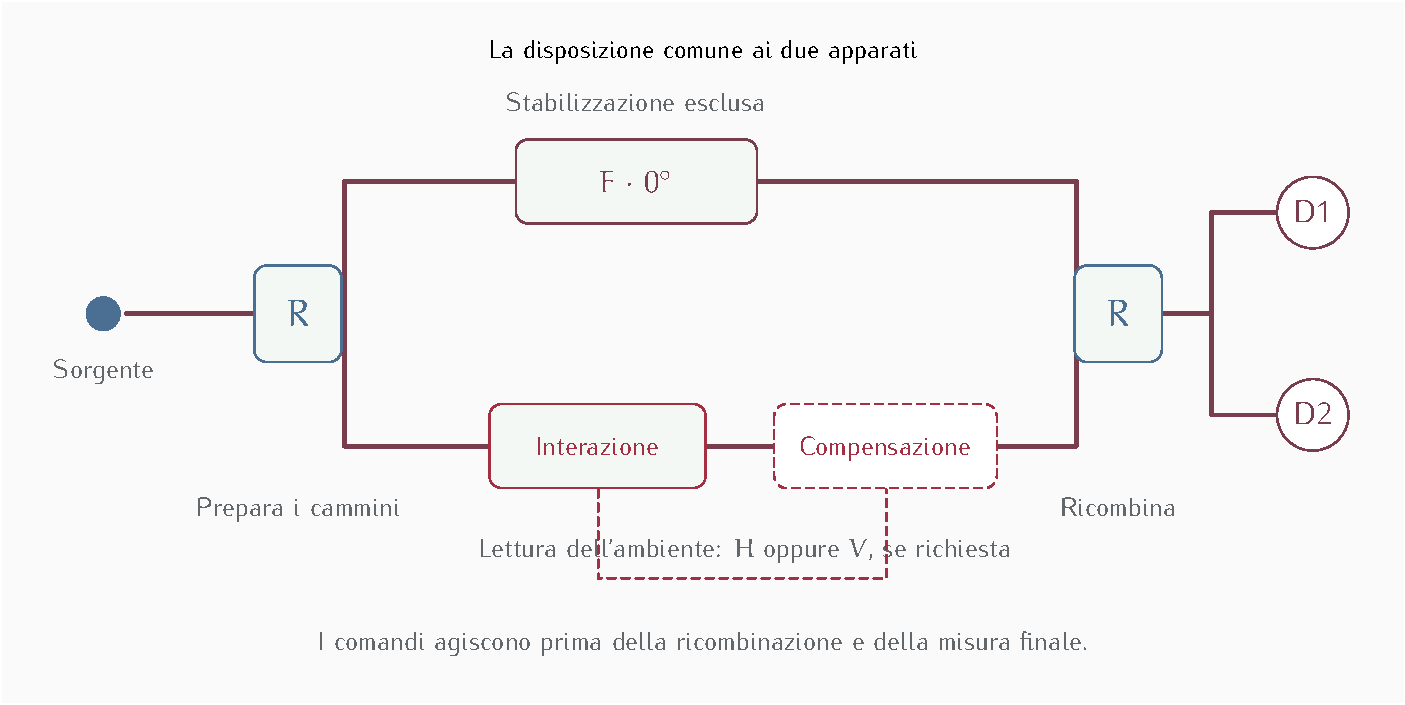
\includegraphics[width=\linewidth,height=94mm,keepaspectratio]{figure/fbb64579c63f10ba0.pdf}\FigureCaption{Disposizione comune ai due apparati: preparazione, due cammini, regolazione della fase, possibile interazione e compensazione, ricombinazione, misura}\end{FigureBlock}


\(R\) prepara i due cammini; \(F\) ne regola la fase relativa. Il riquadro inferiore indica dove un cammino può lasciare una traccia nell'ambiente e dove viene applicata l'operazione inversa. In assenza di marcatura, la compensazione lascia lo stato invariato. \(D_{1}\) e \(D_{2}\) registrano un solo esito a ogni prova.\par

\BookHeading{Variazioni di fase}
La lettura riguarda \(0{}^{\circ} \). La scansione permette di verificare se questa probabilità varia quando cambia la fase.\par

\BookHeading{Tracce dei cammini}
La lettura riguarda \(0{}^{\circ} \). La scansione permette di verificare se questa probabilità varia quando cambia la fase.\par

\BookHeading{Confrontare gli stessi interventi}
Una prima scansione senza interventi fornisce il riferimento. Stabilizzando soltanto la fase e ripetendo la scansione si osserva quale apparato risponde al controllo del ritardo. Il confronto successivo, eseguito con la sola compensazione, verifica il ruolo della traccia nell'ambiente. I pulsanti degli esempi impostano questi casi; i comandi consentono di combinarli liberamente.\par

Prove al secondo\par

Regola soltanto la rapidità della raccolta sullo schermo. Le probabilità di ciascuna prova restano le stesse.\par

\BookHeading{Apparato 1 \(\cdot\) risultati}
La barra colorata mostra la parte della raccolta in cui è comparso ciascun esito: una barra piena corrisponde al 100\%. Il segno verticale indica la probabilità prevista dal modello, anche prima di raccogliere dati.\par

Non sono ancora state eseguite prove. Le barre sono vuote; i segni verticali e le percentuali riportano già ciò che il modello prevede.\par

Ogni prova ripete l'esperimento con una nuova preparazione. Modificare la preparazione o la misura avvia una nuova raccolta: conserva prima il confronto se vuoi ricordare i conteggi precedenti.\par

\BookHeading{Apparato 2 \(\cdot\) risultati}
Non sono ancora state eseguite prove. Le barre sono vuote; i segni verticali e le percentuali riportano già ciò che il modello prevede.\par

\BookHeading{Una scansione completa}
Si raccolgono 2.000 nuove prove a ciascuna delle tredici fasi: 26.000 prove per apparato, 52.000 complessive. I conteggi a fase fissata, mostrati sopra, costituiscono raccolte separate. Nelle curve la coordinata orizzontale è la fase, quella verticale è la frequenza di \(D_{1}\).\par

\BookHeading{Quaderno dei confronti}
Il quaderno conserverà i confronti registrati con il comando accanto alle regolazioni. Per mantenerli anche dopo l'uscita dal laboratorio, esporta il file CSV.\par


\BookHeading{Che cosa mostra questa configurazione}
Entrambi gli apparati prevedono 50/50 per ogni fase nominale.\par

Nell'apparato 1, le variazioni casuali della fase cancellano le frange della raccolta complessiva. Nell'apparato 2, i cammini lasciano tracce distinguibili nell'ambiente. Stabilizzare la fase interviene sulla prima causa; compensare la marcatura interviene sulla seconda. Le curve permettono di seguire separatamente questi effetti, nelle condizioni ideali qui specificate.\par


Il modello e le sue condizioni\par

Apparato 1: interferometro bilanciato senza marcatura, con un ritardo aggiuntivo uniforme su un ciclo completo e indipendente a ogni prova. Per ciascun valore fissato del ritardo è definita una distribuzione con interferenza. Mediando le distribuzioni relative ai diversi ritardi si ottiene probabilità 1/2 in ciascuna uscita. La stabilizzazione elimina questo ritardo aggiuntivo.\par

Apparato 2: fase stabile e marcatura completa, con \(H\) associato al primo cammino e \(V\) al secondo. La compensazione applica l'inversa dell'interazione prima della ricombinazione. Sono modelli ideali specificati, con raccolte indipendenti nei due apparati; l'esperimento verifica le loro previsioni senza fornire una procedura universale per riconoscere ogni possibile ambiente.\par


% Authoritative exercise source. Preserve all derivations and diagrams.

\ExerciseStart{G1.15}{Ricostruire un esperimento a partire dai suoi risultati}{Collegamento}

\BookHeading{Problema, dati e obiettivo}

Due apparati producono entrambi \(P(0)=P(1)=1/2\) dopo un interferometro. In A la fase vale 0 oppure \(\pi\), con uguale frequenza, e l’ambiente non distingue i cammini. In B la fase è stabilmente zero e le tracce ambientali dei cammini sono ortogonali. Progettare due interventi che distinguano le cause.

\ExTheory{\ExRef{c1-sintesi}{1.10}}{Se la sovrapposizione reale delle tracce è \(\gamma\), la probabilità di uscita è \(P(0\mid\varphi)=(1+\gamma\cos\varphi)/2\). Con fasi variabili si media sulle preparazioni. Stabilizzare la fase significa fissare \(\varphi=0\); compensare coerentemente l’interazione ambientale significa riportare \(\gamma\) a 1.}

\ExPrediction{I conteggi iniziali sono uguali. La stabilizzazione dovrebbe cambiare A, mentre la compensazione della traccia dovrebbe cambiare B. L’intervento deve essere eseguito prima della lettura finale.}

\ExFigure{\begin{tikzpicture}[>=Stealth,exlabel]
\node[exbox] (n0) at (0.0,0.0) {A: fase $0/\pi$};\node[exbox] (n1) at (3.6,0.0) {$\gamma=1$};\draw[exother] (n0)--(n1);\node[exbox] (n2) at (7.2,0.0) {$P(0)=1/2$};\draw[exother] (n1)--(n2);\node[exbox] (n3) at (0.0,-1.6) {B: fase $0$};\draw[exother] (n2.south)--++(0,-.4)-|(n3.north);\node[exbox] (n4) at (3.6,-1.6) {$\gamma=0$};\draw[exother] (n3)--(n4);\node[exbox] (n5) at (7.2,-1.6) {$P(0)=1/2$};\draw[exother] (n4)--(n5);
\end{tikzpicture}}{Due preparazioni conducono agli stessi conteggi iniziali.}


\begin{ExTasks}

\item Calcolare i due valori di \(P(0)\) per A e la loro media.

\item Calcolare \(P(0)\) per B.

\item Applicare soltanto la stabilizzazione a entrambi.

\item Applicare soltanto la compensazione ambientale a entrambi.

\item Calcolare il risultato dei due interventi combinati e indicare quali osservazioni distinguano i modelli.

\end{ExTasks}

\ExSolution

\ExStep{Calcolare la media di A}

Per A, \(\gamma=1\). A fase zero \(P(0\mid0)=(1+1)/2=1\); a fase \(\pi\), \(P(0\mid\pi)=(1-1)/2=0\). Quindi
\ExEq{P_A(0)&=\tfrac12\cdot1+\tfrac12\cdot0=\tfrac12.}

\ExStep{Calcolare la previsione di B}

Per B, \(\gamma=0\) e \(\varphi=0\). Pertanto \(P_B(0)=(1+0\cdot1)/2=1/2\). Lo stesso dato finale proviene da una preparazione diversa.

\ExStep{Stabilizzare la fase}

In A si elimina l’alternanza e si fissa \(\varphi=0\): \(P_A(0)=1\). In B la fase era già zero e la traccia resta distinguibile: \(P_B(0)=1/2\). Su 200 prove i conteggi medi di zero sono 200 e 100.

\ExStep{Compensare soltanto la traccia}

In A \(\gamma\) era già 1 e le fasi rimangono alternate: \(P_A(0)=1/2\). In B la compensazione porta \(\gamma=1\) a fase zero: \(P_B(0)=1\). I conteggi medi si scambiano: 100 e 200.

\ExStep{Combinare gli interventi}

Con \(\gamma=1\) e \(\varphi=0\), entrambi danno \(P(0)=(1+1)/2=1\). La coppia ordinata di risposte ai singoli interventi è \((1,1/2)\) per A e \((1/2,1)\) per B: essa discrimina i due modelli ideali. Campioni finiti richiedono confronti statistici coerenti con le incertezze dei conteggi.

\par\noindent\begin{minipage}{\linewidth}
\ExFigure{\begin{tikzpicture}[>=Stealth,exlabel]
\node[exbox] (a) at (0,1) {A};\node[exbox] (b) at (0,-1) {B};\node[exbox] (as) at (4,1) {stabilizza: $1$\ compensa: $1/2$};\node[exbox] (bs) at (4,-1) {stabilizza: $1/2$\ compensa: $1$};\draw[exother] (a)--(as);\draw[exother] (b)--(bs);
\end{tikzpicture}}{Risposte diagnostiche: ogni numero è la probabilità di zero dopo il singolo intervento indicato.}


\ExInterpret{L’identificazione richiede trasformazioni controllate e previsioni confrontabili. La compensazione qui assunta è un’inversione coerente dell’interazione prima della misura; cancellare un dato classico già registrato non realizzerebbe quella trasformazione.}

\ExLab{Nella sezione 1.10 confrontare «Condizioni iniziali», «Stabilizza soltanto la fase», «Compensa soltanto la traccia» e «Applica entrambi gli interventi». Conservare le tabelle dei conteggi e affiancare le probabilità teoriche. I due modelli dell’esercizio fissano i casi ideali cui confrontare i parametri esposti dalla simulazione.}


\end{minipage}


